%% Copernicus Publications Manuscript Preparation Template for LaTeX Submissions
%% ---------------------------------
%% This template should be used for copernicus.cls
%% The class file and some style files are bundled in the Copernicus Latex Package, which can be downloaded from the different journal webpages.
%% For further assistance please contact Copernicus Publications at: production@copernicus.org
%% https://publications.copernicus.org/for_authors/manuscript_preparation.html


%% Please use the following documentclass and journal abbreviations for discussion papers and final revised papers.


%% 2-column papers and discussion papers
\documentclass[acp, manuscript]{copernicus}



%% Journal abbreviations (please use the same for discussion papers and final revised papers)

% Archives Animal Breeding (aab)
% Atmospheric Chemistry and Physics (acp)
% Advances in Geosciences (adgeo)
% Advances in Statistical Climatology, Meteorology and Oceanography (ascmo)
% Annales Geophysicae (angeo)
% ASTRA Proceedings (ap)
% Atmospheric Measurement Techniques (amt)
% Advances in Radio Science (ars)
% Advances in Science and Research (asr)
% Biogeosciences (bg)
% Climate of the Past (cp)
% Drinking Water Engineering and Science (dwes)
% Earth System Dynamics (esd)
% Earth Surface Dynamics (esurf)
% Earth System Science Data (essd)
% Fossil Record (fr)
% Geographica Helvetica (gh)
% Geoscientific Instrumentation, Methods and Data Systems (gi)
% Geoscientific Model Development (gmd)
% Geothermal Energy Science (gtes)
% Hydrology and Earth System Sciences (hess)
% History of Geo- and Space Sciences (hgss)
% Journal of Micropalaeontology (jm)
% Journal of Sensors and Sensor Systems (jsss)
% Mechanical Sciences (ms)
% Natural Hazards and Earth System Sciences (nhess)
% Nonlinear Processes in Geophysics (npg)
% Ocean Science (os)
% Proceedings of the International Association of Hydrological Sciences (piahs)
% Primate Biology (pb)
% Scientific Drilling (sd)
% SOIL (soil)
% Solid Earth (se)
% The Cryosphere (tc)
% Web Ecology (we)
% Wind Energy Science (wes)


%% \usepackage commands included in the copernicus.cls:
%\usepackage[german, english]{babel}
%\usepackage{tabularx}
%\usepackage{cancel}
%\usepackage{multirow}
%\usepackage{supertabular}
%\usepackage{algorithmic}
%\usepackage{algorithm}
%\usepackage{amsthm}
%\usepackage{float}
%\usepackage{subfig}
%\usepackage{rotating}


\begin{document}

\title{Emissions of trace gases from Australian temperate forest fires: emission factors and dependence on modified combustion efficiency}


% \Author[affil]{given_name}{surname}

\Author[1]{Elise-Andr\'ee}{Gu\'erette}
\Author[1]{Clare}{Paton-Walsh}
\Author[1]{Maximilien}{Desservettaz}
\Author[2]{Thomas E.L}{Smith}
\Author[3]{Liubov}{Volkova}
\Author[3]{Christopher J.}{Weston}
\Author[4]{C.P. (Mick)}{Meyer}

\affil[1]{Centre for Atmospheric Chemistry, School of Chemistry, University of Wollongong, Wollongong, NSW, Australia}
\affil[2]{Department of Geography, King's College London, London, UK}
\affil[3]{School of Ecosystem and Forest Sciences, the University of Melbourne, Creswick, VIC, Australia}
\affil[4]{CSIRO Oceans and Atmosphere Flagship, Aspendale, VIC, Australia}

%% The [] brackets identify the author with the corresponding affiliation. 1, 2, 3, etc. should be inserted.



\runningtitle{Emissions of trace gases from Australian temperate forest fires}

\runningauthor{Guerette et al.}

\correspondence{E-A. Gu\'erette (eag873@uowmail.edu.au)}



\received{}
\pubdiscuss{} %% only important for two-stage journals
\revised{}
\accepted{}
\published{}

%% These dates will be inserted by Copernicus Publications during the typesetting process.


\firstpage{1}

\maketitle



\begin{abstract}
We characterised trace gas emissions from Australian temperate forest fires through a mixture of in situ open-path FTIR measurements spectroscopy and selective ion flow tube mass spectrometry (SIFT-MS) and White cell FTIR spectroscopy of grab samples. We report emission factors for a total of 25 trace gas species measured in smoke from nine prescribed fires. We find significant dependence on modified combustion efficiency (MCE) for some species, although regional differences indicate that the use of MCE as a proxy may be limited. We also find that the fire-integrated MCE values derived from our in situ on-the-ground open-path measurements are not significantly different from those reported for airborne measurements of smoke from fires in the same ecosystem. We then compare our average emission factors to those measured for temperate forest fires elsewhere (North America) and for fires in another dominant Australian ecosystem (savanna) and find significant differences in both cases. Indeed, we find that although the emission factors of some species agree within 20$\%$, including those of hydrogen cyanide, ethene, methanol, formaldehyde and 1,3-butadiene; others, such as acetic acid, ethanol, monoterpenes, ammonia, acetonitrile and pyrrole, differ by a factor of two or more. This indicates that the use of ecosystem-specific emission factors is warranted for applications involving emissions from Australian forest fires.  
\end{abstract}


%\copyrightstatement{TEXT}


\introduction  %% \introduction[modified heading if necessary]
Biomass burning emits a wide range of trace species, including greenhouse gases, particulate matter and volatile organic compounds (VOCs). Globally, fires are the second largest source of VOCs, with emissions estimated at 400 Tg yr$^{-1}$ on average \citep{Yokelson2008,Akagi2011}. Fires are also the main driver of inter-annual variability for species such as carbon monoxide and particulate matter \citep{Edwards2004,Edwards2006,Voulgarakis2015}.  

Australia emits 7-8 $\%$ of global annual biomass burning carbon emissions \citep{Ito2004,VanderWerf2010}. At a national level, average gross annual emissions of total carbon from fires (127 Tg C yr$^{-1}$) actually exceed those from burning fossil fuels (95 Tg C yr$^{-1}$) \citep{Haverd2013}. While net emissions of carbon from fires are lower due to regrowth \citep{Haverd2013, Landry2016}, volatile organic species emitted by those fires are not subject to uptake by the regenerating vegetation and can therefore be considered net emissions. 

The mix of VOCs emitted during biomass burning may be ecosystem-specific, with species such as monoterpenes being distilled from the vegetation as it is heated by the approaching fire \citep{Ciccioli2014}. Methanol, acetic acid, acetaldehyde, acetone and monoterpenes have all been detected from heated \textit{Eucalyptus} leaves in laboratory experiments, with differences observed between fresh leaves and senescent leaves \citep{Greenberg2006,Maleknia2007,Maleknia2009,Possell2013}. Other factors that impact smoke composition include fuel composition \citep[e.g. nitrogen content,][]{Coggon2016} and fire behaviour \citep[e.g.][]{Wooster2011}. %and fuel moisture \citep[e.g.][]{Hoffa1999}. 
Changes in fire behaviour can be reflected in the combustion efficiency of the fire, i.e. in the proportion of total carbon that is emitted as CO$_2$. A useful proxy for combustion efficiency is modified combustion efficiency (MCE), which is defined as the ratio of CO$_2$ released to the sum of CO and CO$_2$ \citep{Hao1993,Yokelson1996}. Emission factors of several trace gases have been found to correlate to MCE in a number of ecosystems \citep[e.g.][]{Akagi2013, Burling2011, Meyer2012}.

The composition of fresh smoke matters as it affects plume chemistry as the smoke ages, contributing to varying rates of ozone and aerosol formation \citep{Yokelson2009,Akagi2012,Alvarado2015} and elevated ozone and particulates downwind of the fires \citep{Pfister2008,Yan2008}.

Most of the area burnt in Australia annually is in the semi-arid and tropical savannas in the north of the country \citep{Russell-Smith2007}, but large bushfires also occur regularly in the temperate forests that cover extensive areas of the south-east of Australia \citep{Cai2009}. These fires can be intense enough to create pyro-convective lofting and inject smoke at high altitudes \citep{Fromm2006,Dirksen2009,Guan2010,Siddaway2011,DeLaat2012} and are expected to become more frequent under a changing climate \citep{Bradstock2009,Cai2009,Keywood2013,King2013}. There has been growing interest in characterising the composition of smoke from Australian temperate forest fires in recent years, mostly arising from increased awareness of the significant impacts of bushfire smoke on regional air quality \citep{Reisen2011,Reisen2013,Price2012,Keywood2015,Rea2016} and its associated repercussions on human health \citep{Reisen2006,Johnston2012,Johnston2014, Reisen2015, Reid2016}, coincident with a mandate for state agencies to increase prescribed burning in the wake of the catastrophic 2009 forest fires in Victoria \citep{Teague2010}. Prescribed burning is widely used in Australia as a means of reducing bushfire risk \citep{Boer2009}; however, these low to moderate intensity fires often take place close to population centres, under weather conditions (low wind speeds, stable atmosphere) that are conducive to pollution build up, sometimes on a regional scale \citep[e.g.,][Fig. 2]{Williamson2016}, with potential health impacts on nearby population \citep{Haikerwal2015}.

Most of what is known about the VOC emissions from Australian temperate fires to date comes from opportunistic measurements of bushfire plumes impacting measurement sites such as the University of Wollongong \citep{Paton-Walsh2005,Paton-Walsh2008, Rea2016} or the Cape Grim Baseline Air Pollution Station \citep{Lawson2015} or captured from space using satellite sensors \citep{Young2011,Glatthor2013}. Dedicated field and laboratory measurement campaigns have mostly focused on greenhouse gases \citep{Hurst1996,Volkova2014, Possell2015, Surawski2015}.

\citet{Volkova2014} reported emission factors for carbon dioxide (CO$_2$), carbon monoside (CO), methane (CH$_4$) and nitrous oxide (N$_2$O) separately for burning fine fuels and logs from measurements made on the ground at prescribed fires in the State of Victoria. \citet{Surawski2015} measured emissions of CO$_2$, CO, CH$_4$ and N$_2$O from fine \textit{Eucalyptus}
 litter fuels in a combustion wind tunnel and found that emissions from these fuels vary depending on the mode of fire spread and on the phase of combustion. \citet{Possell2015} reported emission factors for CO$_2$ and CO for several fuel classes combusted in a mass-loss calorimeter and estimated the total fraction of fuel carbon that would be emitted as CH$_4$, particulates and non-methane hydrocarbons using a carbon mass balance approach. The only whole fire emission factors available are those from \citet{Hurst1996}, who sampled smoke plumes from fires in the greater Sydney region from an aircraft and reported emission factors for CO$_2$, CO and CH$_4$. 

This paper presents results from a dedicated ground measurement program that sampled smoke at several prescribed fires organised by the New South Wales (NSW) National Parks and Wildlife Service in the greater Sydney area and by the Department of Environment, Land, Water and Planning %(DELWP)
in the State of Victoria. Measurements made at a subset of these fires were presented in \citet{Paton-Walsh2014} along with a detailed description of the open-path Fourier Transform Infrared system (OP-FTIR) and a discussion of the uncertainties associated with deriving emission factors using this technique.
Here, we present emission factors for 15 additional VOC species, measured by selected ion flow tube mass spectrometry (SIFT-MS) from grab samples collected at prescribed fires in NSW, as well as additional OP-FTIR results from fires in the State of Victoria.
We then investigate the dependence of the measured emission factors on MCE, using all the data collected to date. We also compare the average MCE values observed in our ground measurements to MCE values reported for measurements from other platforms, including airborne measurements. Finally, we compare our average emission factors to values reported in the literature for other ecosystems. Currently, widely used compilations of emission factors \citep[e.g.,][]{Akagi2011} do not include any results from Australian forests fires. In fact, the emission factors listed for temperate forests in \citet{Akagi2011} are sourced exclusively from measurements made at North American fires. We compare our results with the emission factors listed in \citet[Table S4, February 2015 update]{Akagi2011} for temperate forests and to emission factors measured for Australian savanna fires \citep{Smith2014} and find significant differences in both cases. %We therefore conclude that the use of ecosystem-specific emission factors for Australian forest fires is warranted.   

\section{Methods}
%TEXT
\subsection{Prescribed fires}


\begin{figure}
  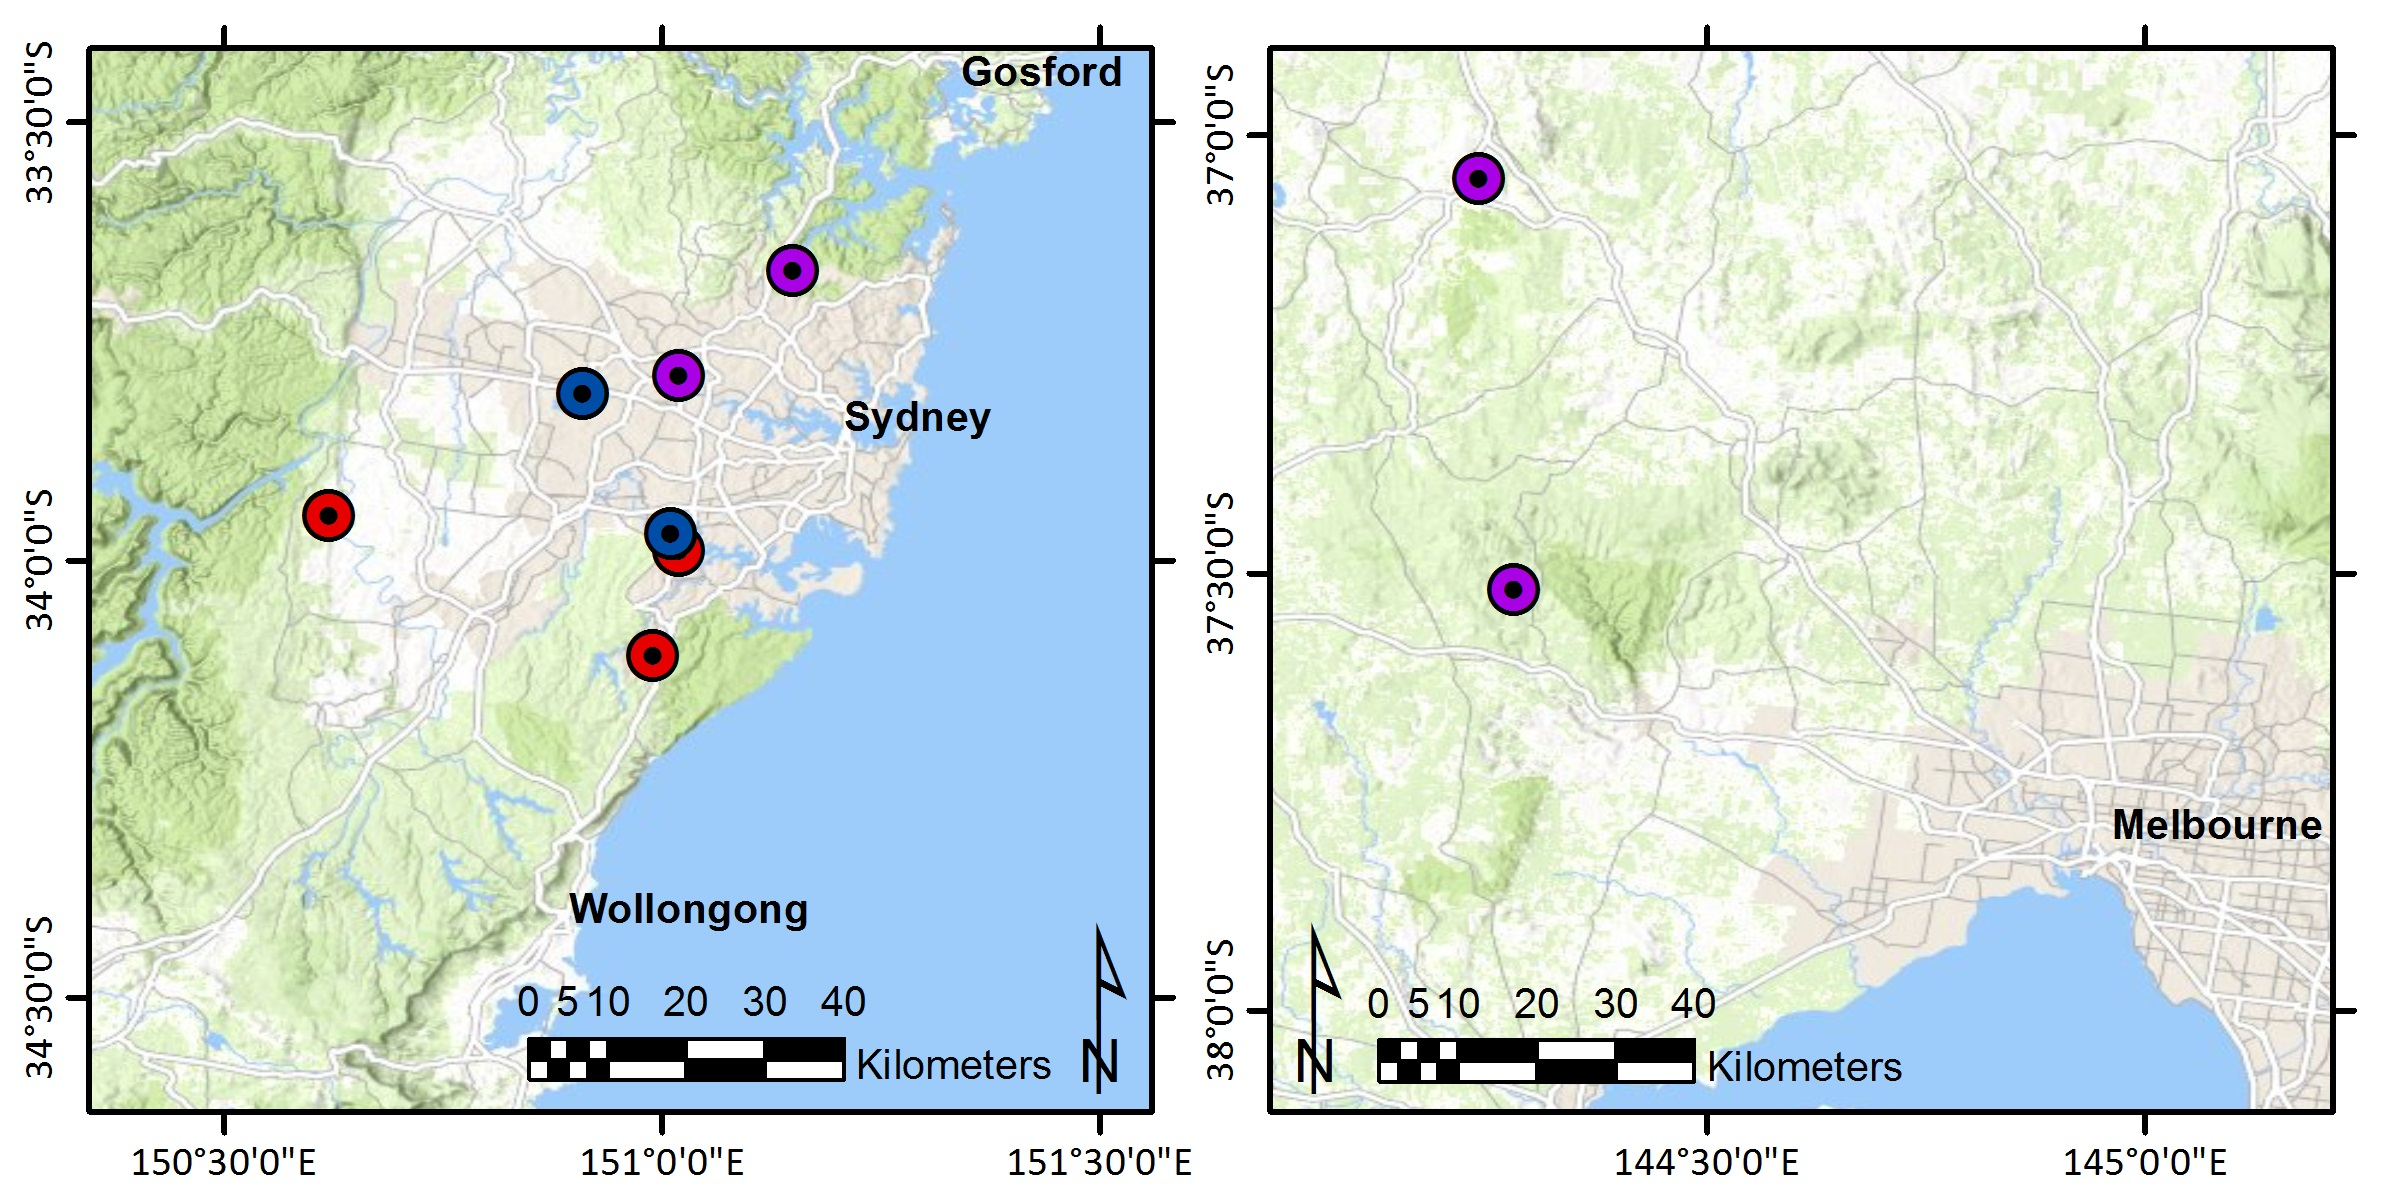
\includegraphics[width=14 cm]{C:/Users/eag873/Documents/GitHub/HRB_paper/figures/Elise_Figure1.png}
  \caption{Locations of the nine prescribed fires in Australian temperate forests sampled between 2010 and 2015. The NSW fires are on the left, and the fires in Victoria on the right. The red dots represent fires where both open-path FTIR (OP-FTIR) and grab sampling took place, the blue dots indicate fires where only grab sampling took place, and the purple dots indicate fires where only OP-FTIR sampling took place.}
  \label{fig:map}
\end{figure}

Between 2010 and 2015, we sampled a total of nine prescribed fires in Australian temperate forests. Seven of those fires took place in New South Wales (NSW) in 2010-2013, the other two fires were sampled in the State of Victoria in April 2015. The locations of the fires sampled are indicated on the maps shown in Fig.~\ref{fig:map}. All fires took place in variants of dry sclerophyll forests, dominated by eucalypt species. Table S1 lists the fires, their location, the dates on which they were sampled, the main vegetation type, the area burnt, the fuel loading, the time elapsed since the previous fire, the coordinates of the sampling sites and the method(s) of sampling deployed (these methods correspond to the colour coding on the maps in Fig.~\ref{fig:map}). 

In NSW, all fires took place in the Greater Sydney area, as seen in Fig.~\ref{fig:map}. Dominant overstorey species included eucalypts (including \textit{Eucalyptus}, \textit{Corymbia} and \textit{Angophora} species), with \textit{Melaleuca}, \textit{Acacia} and \textit{Banksia} species in the sub-canopy and the shrubby understorey. The ground cover was generally made up of native grasses and a litter of eucalypt leaves, bark and twigs, as well as fallen tree limbs of varying sizes.
 
In Victoria, dominant overstorey species were \textit{E. radiata} (Sieb. ex. DC.), \textit{E. obliqua} (L'H\'erit.), \textit{E. dives} (Schau.), \textit{E. leucoxylon} (F. Muell.) 
and \textit{E. macrorhyncha} (F. Muell.). \textit{Acacia} and \textit{Banksia} species dominated the understorey. Ground cover was dominated by tree litter, with gorse (\textit{Ulex europaeus}) and blackberry (\textit{Rubus fruticosus}) recorded in some areas.


\subsection{Open-path FTIR system (OP-FTIR)}


An open-path FTIR system was deployed at five prescribed fires in NSW and at the two prescribed fires in Victoria, as indicated in the last column of Table S1. The system used in this project is described in detail in \citet{Paton-Walsh2014}. Briefly, the spectrometer (Bomem MB-100 Series, 1 cm$^{-1}$ resolution) has a built-in infrared source and is placed 20-50 meters away from a set of retro-reflectors positioned so that smoke from the fire crosses the path in between. The system can run autonomously and records a spectrum consisting of three scans, approximately every twenty seconds. Ambient pressure and temperature are monitored at one end of the path, through a barometer (Vaisala PTB110) and a resistance temperature detector (RTD PT100) connected to the computer controlling the spectrometer via an I/O box. The output is logged at the same time resolution as the spectral measurements. 
%Ambient pressure is not expected to vary much along the measurement path, however temperature may be significantly affected by flames crossing the path. This is considered in the uncertainty budget developed by \citet{Paton-Walsh2014} for the OP-FTIR measurements of emission factors.  

Typically, the system is set up and starts recording before the fire is ignited, and is left to run until mole fractions return to ambient values. As the measurement is integrated over a path of several meters and is continuous over the duration of the fire, the emissions measured using this technique are likely to capture smoke from all stages of the fire, and therefore to be representative of the whole fire. One of the great advantages of OP-FTIR is that there is no sample capture, avoiding losses due to walls or sample lines. 

In April 2015, the OP-FTIR was deployed at two prescribed burns in temperate forests in Victoria, several hundred kilometres away from the fires sampled in 2010-2013. The first fire, on April 13$^{th}$, was near Greendale, Victoria, and the second, on April 23$^{rd}$, was in Kalimna Park, Castlemaine, Victoria (see Fig.~\ref{fig:map} for a map of the locations). At the Greendale fire, the spectrometer was positioned along a fire trail and the retro-reflectors were installed 45 m away within the woodland area to be burned, so that both smoke and flames passed through the line of sight of the instrument. At the Castlemaine fire, both the spectrometer and the retro-reflectors were positioned along a fire trail downwind of the fire, so that smoke would blow through the 50 m measurement path. The instrument set-up at both fires is shown in Fig.~\ref{fig:OP}. The details of the NSW deployments are in \citet{Paton-Walsh2014}. 

The OP-FTIR spectra collected during the fires were subsequently analysed to derive mole fractions of carbon dioxide (CO$_2$), carbon monoxide (CO), methane (CH$_4$), acetic acid (CH$_3$COOH), ammonia (NH$_3$), ethene (C$_2$H$_4$), formaldehyde (H$_2$CO), formic acid (HCOOH) and methanol (CH$_3$OH) using the Multiple Atmospheric Layer Transmission (MALT) model \citep{Griffith1996,Griffith2012} and the spectral windows described in \citet{Paton-Walsh2014}. The uncertainty on individual measurements is the error on the retrieval reported by MALT. For a complete uncertainty budget for the OP-FTIR measurements in smoke, see Appendix B of \citet{Paton-Walsh2014}.

\begin{figure}
  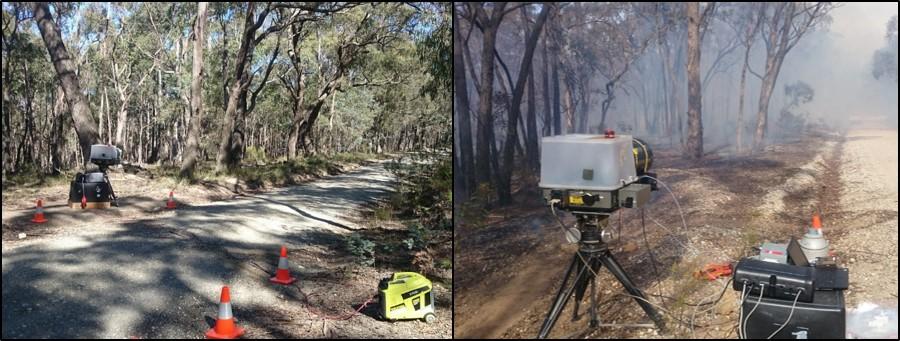
\includegraphics[width=14cm]{C:/Users/eag873/Documents/GitHub/HRB_paper/figures/OP.jpg}
  \caption{The instrumental set-up for the open-path FTIR measurements of smoke at Greendale on April 13$^{th}$, 2015 (left) and Castlemaine on April 23$^{rd}$, 2015 (right).}
  \label{fig:OP}
\end{figure}

\subsection{Grab sampling}
A total of 67 smoke samples were collected over seven days of sampling at five prescribed fires in NSW. Of those samples, over half were of well mixed, rising smoke. The others were from various targets, including smouldering litter and logs and burning grass and shrubs. The number of samples collected at each fire is indicated in brackets in the last column of Table S1. 
Samples were collected in 600 ml glass flasks, except at the Gulguer Plateau fire, where samples were collected into 1 L Tedlar bags. The glass flasks were pre-evacuated using a turbo-molecular pump (Pfeiffer TCS 010) prior to deployment to the fires, and filled with smoke on site by opening them for a few seconds. No sample line was affixed to the flasks for sampling; flasks were positioned in the smoke prior to opening them. The bags were flushed with high purity nitrogen and brought to the Gulguer Plateau fire where they were filled with smoke using a differential pressure system or 'vacuum box' powered by a generator. As the generator had to be placed away from the fire, a sample line ($\sim$5 meters) was attached to the vacuum box. Filling the bags took a few minutes, and consequently, most samples were collected from large smouldering targets after the fire front had moved through the sampling area. 

All grab samples were brought back to the lab and analysed within 24 hours of collection. A Fourier Transform Infrared (FTIR) spectrometer coupled to a White cell was used to measure carbon dioxide (CO$_2$), carbon monoxide (CO), methane (CH$_4$), ethane (C$_2$H$_6$) and ethene (C$_2$H$_4$). VOC mole fractions were measured using selective ion flow tube mass spectrometry (SIFT-MS).


\subsubsection{Fourier Transform Infrared (FTIR) spectrometer coupled to a White cell (White cell FTIR)}
Mole fractions of CO$_2$, CO, CH$_4$, C$_2$H$_6$ and C$_2$H$_4$ in the grab samples of smoke collected at the fires were measured using a Bomem MB-100 Series FTIR spectrometer (1 cm$^{-1}$ resolution). This spectrometer is coupled to a multi-pass optical (White) cell with a path of 22.2 m and is fitted with an indium antimony (InSb) detector cooled with liquid nitrogen. 

Part of the sample was transferred to the evacuated White cell and the temperature and pressure inside the cell were logged. Typical temperatures and pressures inside the White cell were 22$^\circ$C and 220 hPa, respectively. A spectrum consisting of 78 scans was acquired for each grab sample. Mole fractions were retrieved using the Multiple Atmospheric Layer Transmission (MALT) model \citep{Griffith1996,Griffith2012}. The uncertainty on individual grab sample measurements is taken as the error reported by MALT for the retrieval. 
 

\subsubsection{Selective Ion Flow Tube Mass Spectrometry (SIFT-MS)}
SIFT-MS is a technique for the on-line analysis of gas samples that is akin to the better-known Proton-Transfer-Reaction Mass Spectrometry (PTR-MS) \citep{Blake2009}. Both instruments use chemical ionization to ionize the VOCs present in air and both are equipped with quadrupole mass filters. The main advantage of SIFT-MS is its capability to switch between three reagent ions (H$_3$O$^+$, NO$^+$ and O$_{2}^+$) within a single measurement cycle, allowing the detection of species such as acetylene and ethene in addition to the species commonly detected using PTR-MS within the same analysis. It does this by producing all three reagent ions simultaneously in a microwave discharge and then selecting one or the other (switching) using a quadrupole mass filter (the instrument therefore has two quadrupole mass filters). By contrast, PTR-MS is typically equipped with a hollow-cathode discharge that produces a pure stream of a single reagent ion (most commonly H$_3$O$^+$) and therefore requires a single quadrupole. 
Another difference is that PTR-MS uses a drift tube as its reaction chamber (in which ions are carried by an electric field), whereas SIFT-MS is equipped with a flow tube. The specific instrument used in this study (Syft Voice 100) uses a stream of helium and argon to thermalize and carry the ions \citep{Milligan2007}. 
This means that the instrument dilutes the sample by a factor that is a function of the pressure and temperature inside the flow tube, and of the flows of sample and carrier gases. This makes the instrument less sensitive than PTR-MS \citep{Blake2009} but ideally suited for the analysis of highly polluted air, such as smoke samples. The flow tube dilution ratio under standard operating conditions is about 1:15.  

The SIFT-MS was operated in multiple ion mode, targeting eighteen VOC species. Table S2 lists the species targeted, the reagent ion used, the mass-to-charge ratios measured and the calibration factors used to quantify them. The list includes aromatic species, nitrogen-containing species, some oxygenated species, some small hydrocarbons and some biogenic species, targeting a breadth of chemical classes. The species targeted were for the most part the most abundant reported at their nominal molecular mass by \citet{Yokelson2013}, who deployed extensive instrumentation in a laboratory setting and calculated emission factors for 357 species. A notable exception is the signal at NO$^+$ 68, which is calibrated using isoprene, but is expected to be dominated by furan in smoke samples. Also, the signal at H$_3$O$^+$ 71 is expected to include 2-butenal as well as methacrolein (MACR) and methyl vinyl ketone (MVK). 
The measurement cycle took approximately 7 seconds to complete and was repeated 8 times on each smoke sample. Mole fractions of VOCs were computed from raw SIFT-MS spectra using the calibration factors listed in Table S2. For each sample, an average mole fraction was calculated for each species by taking the mean over all repeats. The standard deviation of the mean was taken as the uncertainty on the average mole fraction. An average mole fraction was reported for a given species only if its signal-to-noise ratio was greater than three, i.e. if the average signal was at least three times greater than the standard deviation of its mean. 

\begin{figure}[t]
  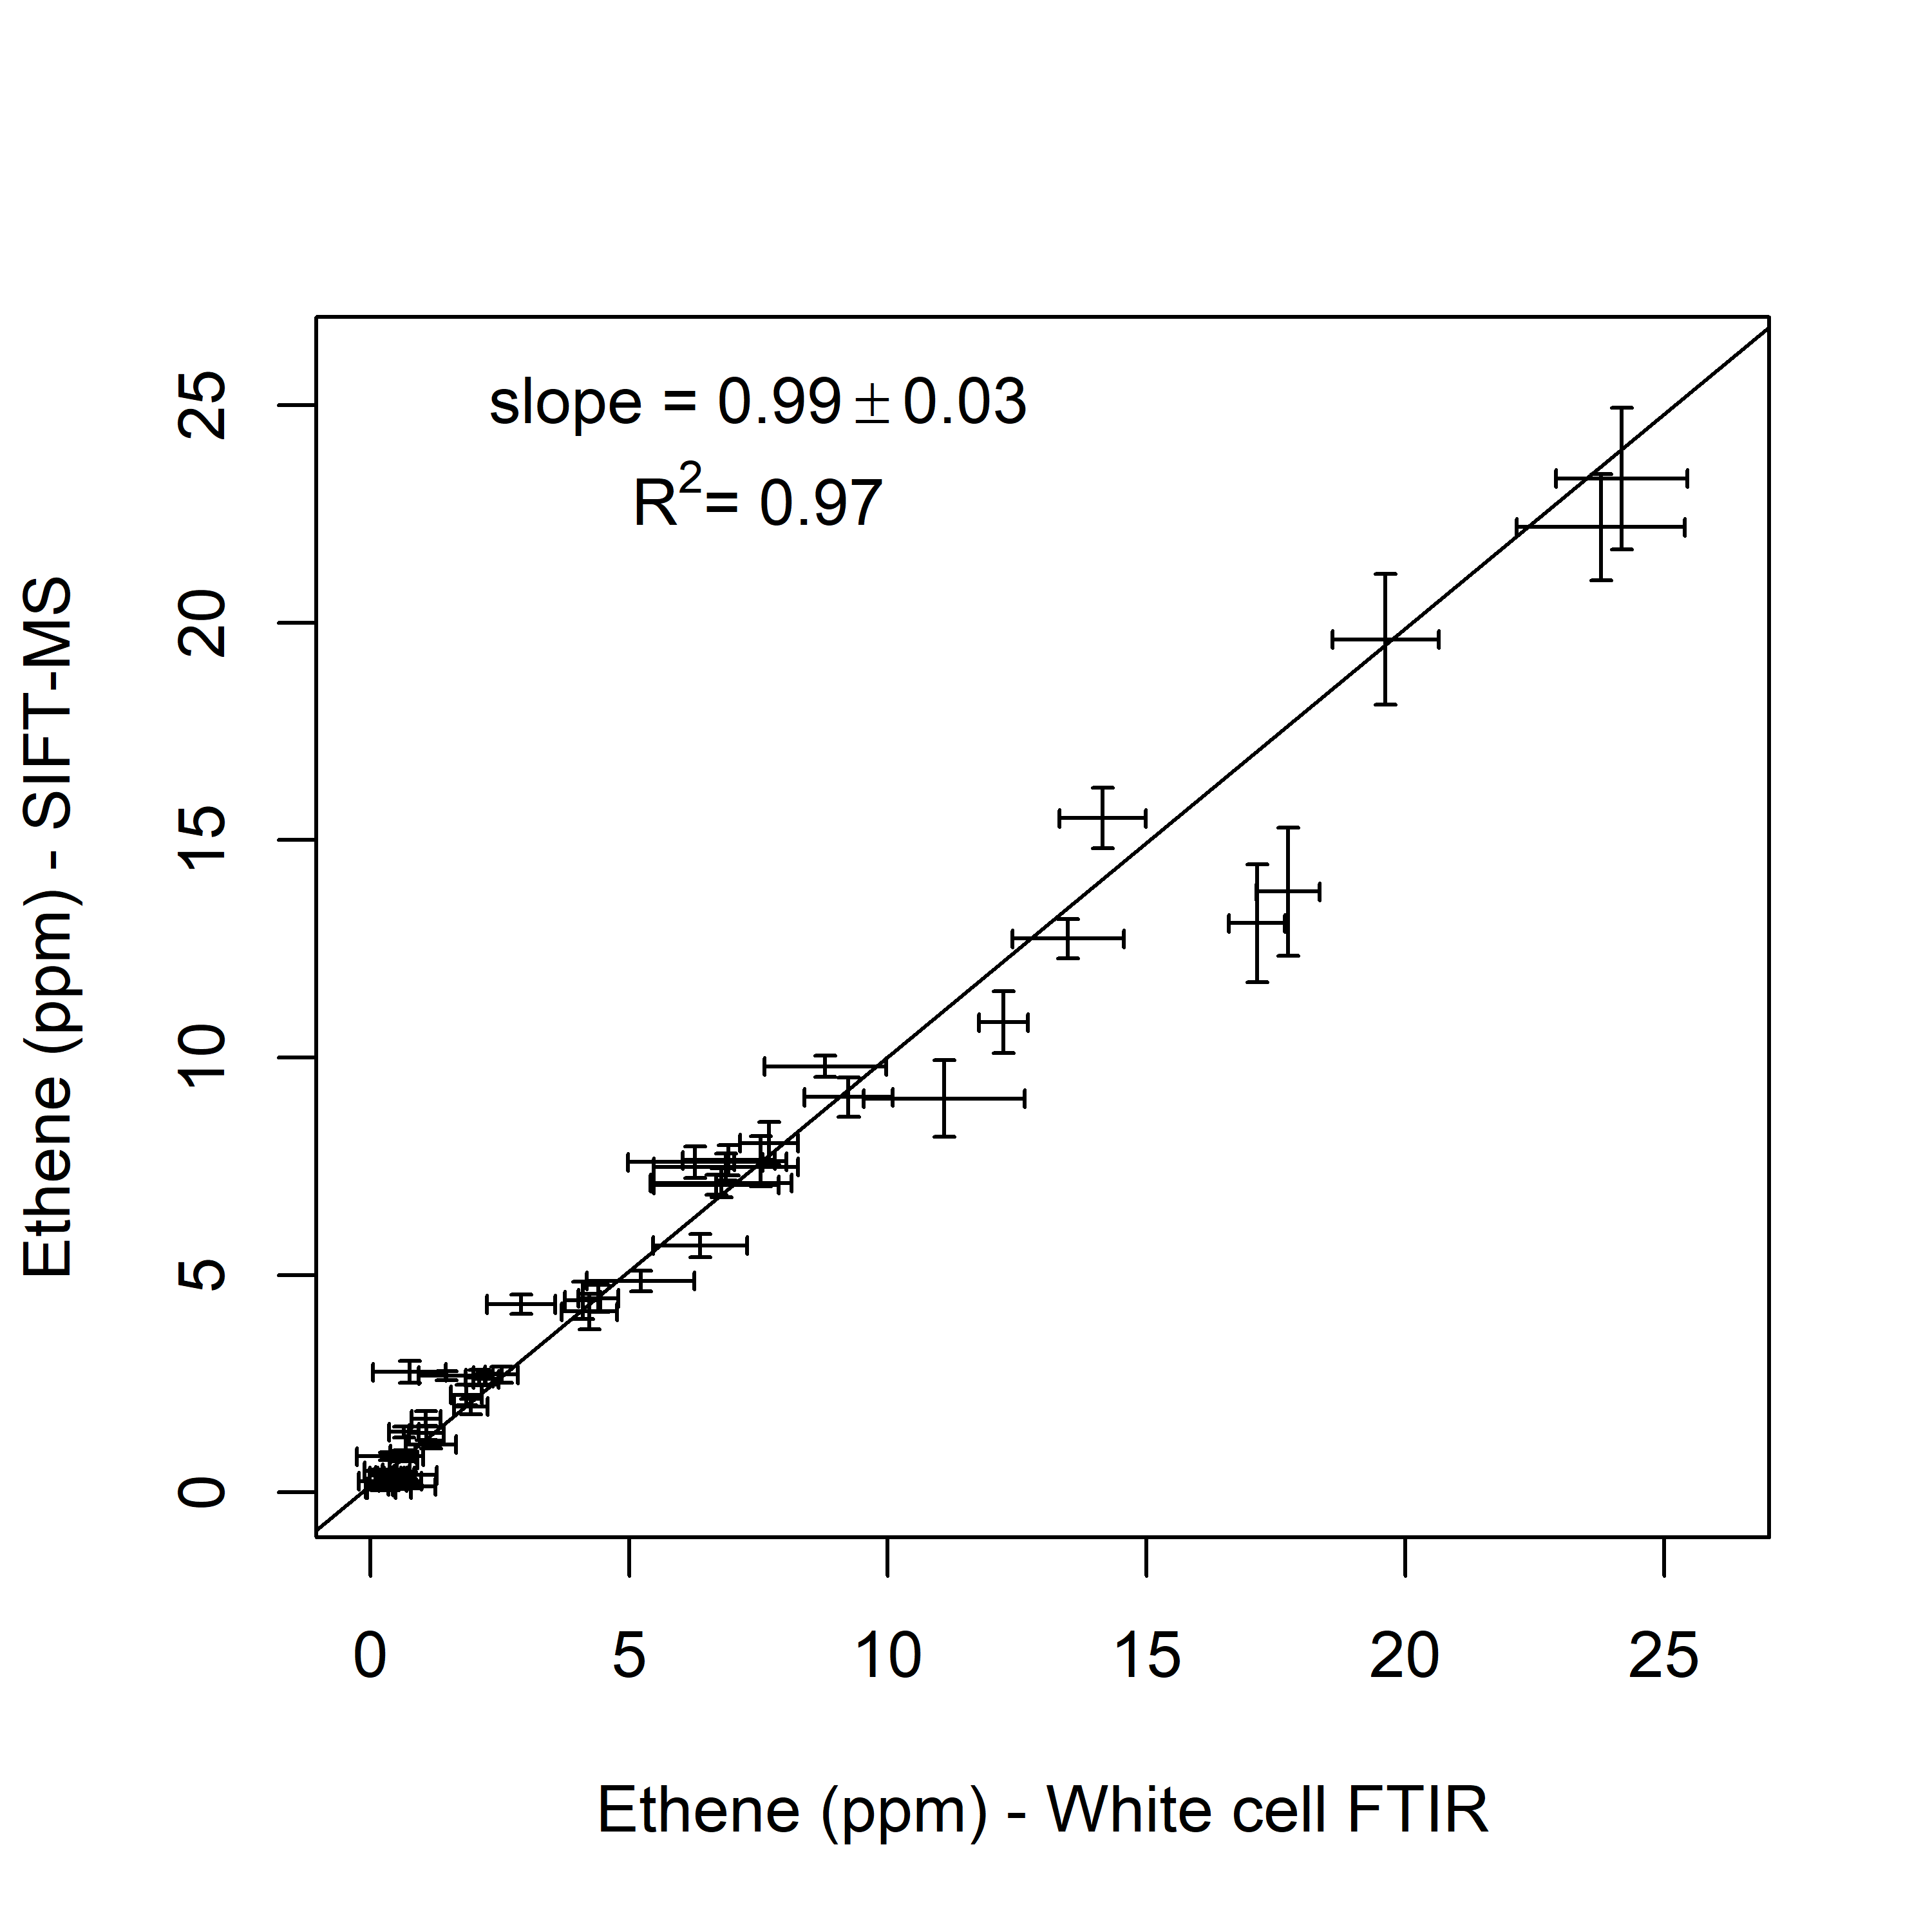
\includegraphics[width=8.3 cm]{C:/Users/eag873/Documents/GitHub/HRB_paper/figures/Ethene_w_error_bars_bigger_no_pts.png}
  \caption{Comparison of ethene mole fractions measured by SIFT-MS with those measured by White cell FTIR in grab samples of smoke collected at Australian temperate forest fires. Error bars for the SIFT-MS are the standard deviation of the measurement, for the White cell FTIR they are the error on the retrieval. The line of best fit was determined using orthogonal regression.
  }
  \label{fig:ethene}
\end{figure}

The linearity of the SIFT-MS response was checked by plotting the mole fractions measured for ethene against those measured by White cell FTIR in the same grab samples. Figure \ref{fig:ethene} shows the good agreement for ethene between the two methods. The plot demonstrates that there was no loss of linearity in the SIFT-MS response even at high mole fractions, which is a result of the sample dilution that occurs within the flow tube of the instrument.

\subsection{Determination of emission ratios (ER)} \label{sec:ER_calc}
Emission ratios (ER) were derived by plotting VOC mole fractions against those of CO or CO$_2$ (or another reference VOC species in some cases, see below) and applying an orthogonal regression. Orthogonal regression finds the best line of fit by minimising squared distances between (x, y) points and their projection on the line of best fit. The regression is also weighted by the uncertainties in both x and y, which, in this case, are the measurement uncertainties described above, so that the line of best fit has greater dependence on the more precise data points. The slope of the line of best fit is the emission ratio. As noted in a recent evaluation of linear regression techniques \citep{Wu2017}, the type of linear regression applied has little impact on the resulting slope as long as the correlation coefficient is high. For this reason, we chose pairs of species that were well correlated to derive emission ratios and do not report results when R$^2$ < 0.5, as this should yield the most robust results. More generally, we chose to use linear regression to derive ER instead of calculating a value from each measurement \citep[e.g.][]{Burling2011} because the background mole fractions of many measured species were poorly defined, often being below the detection limit of the SIFT-MS. Deriving emission ratio through regression without first subtracting background values introduces very little error \citep[< $0.1 \%$,][]{Wooster2011}.

Emission ratios were derived from the open-path measurements for each fire separately. The mean ER from all the fires sampled is then our best estimate for the ecosystem. For the grab samples, emission ratios were derived for individual fires when possible; however, the VOC results from the targeted grab sampling were more highly variable than the open-path measurements in the well-mixed smoke, as is common for this type of sampling \citep{Yokelson2008,Yokelson2013,Burling2011,Akagi2013}. This resulted in poor correlations (R$^2$ < 0.5) for some species for certain fires. Also, not every trace gas species was present at a detectable level in every sample. For some fires, this resulted in too few samples to allow an emission ratio to be meaningfully derived by regression for that species. As ER were not successfully derived for each fire for some species, a mean ER was not necessarily the best estimate for the ecosystem. To derive a best estimate for the ecosystem, all valid samples were combined irrespective of which fire they were collected at and a single ER derived through orthogonal regression. 
Certain VOC species measured in the grab samples did not correlate strongly with either CO or CO$_2$. In those cases, emission ratios were derived using another reference species, e.g. an emission ratio to acetonitrile was derived for pyrrole, and ethene was used as a reference species to derive an emission ratio for benzene, 1,3-butadiene and acetylene. Good correlation between VOC species may indicate co-emission. 

\subsection{Determination of emission factors (EF) and modified combustion efficiency (MCE)}
An emission factor (EF) is defined as the mass of trace gas of interest (X) released per amount of dry biomass burnt and is typically expressed in units of g kg$^{-1}$:
\begin{equation} \label{eq:EF:mass_ratio}
EF_X = 1000 \times \frac{mass_X}{mass_{dry fuel burnt}}
\end{equation}

This is a very direct method of estimating emissions, but can only be used if all the emissions are captured (so that the total mass of gas X can be measured) and if the mass of biomass burnt in the fire is known \citep{Andreae2001}, which is rarely the case except in laboratory experiments. In the absence of such knowledge, the total mass of biomass burnt can be derived from the total mass of carbon emitted and the fractional carbon content of the biomass burnt (F$_{carbon}$), which is sometimes measured but often estimated:

\begin{equation} \label{eq:EF:Fc_mass_ratio}
EF_X = F_{carbon} \times 1000 \times \frac{mass_X}{mass_{dry fuel burnt}}
\end{equation}

In this study, F$_{carbon}$ was assigned a value of 0.5, as in \citet{Akagi2011},\citet{Yokelson2011} and \citet{Paton-Walsh2014}. Similarly, the total mass of carbon emitted by a fire is usually not known, and is estimated by measuring the most abundant carbon-containing species emitted by the fire. The emission factor for species X is then:

\begin{equation} \label{eq:EF:cx_ct}
EF_X = F_{carbon} \times 1000 \times \frac{MM_X}{12} \times \frac{C_X}{C_T}
\end{equation}

where MM$_X$ is the molar mass of the species of interest, 12 is the atomic mass of carbon and $ \frac{C_X}{C_T} $ is the number of moles of species X emitted divided by the total number of moles of carbon emitted. In general, only a subset of the smoke from a fire is sampled. If that sample is representative of the whole fire, then the observed ratio of a species to the sum of all other species  $ \frac{C_X}{C_T} $ should be representative of the entire fire.  $ \frac{C_X}{C_T} $ can be calculated directly from the excess amounts measured:

\begin{equation} \label{eq:EF:delta_ratio}
EF_X = F_{carbon} \times 1000 \times \frac{MM_X}{12} \times \frac{\Delta[X]}{\sum_{y=1}^{n} NC_y \times \Delta[Y]}
\end{equation}

where $\Delta[X]$ and $\Delta[Y]$ are the total excess mole fraction of the species of interest and of another carbon-containing species, respectively, NC$_y$ is the number of carbon atoms in species Y and the sum is over all carbon-containing species measured in the smoke. 
Equation \ref{eq:EF:delta_ratio} can also be written as:

\begin{equation}
EF_X = F_{carbon} \times 1000 \times \frac{MM_X}{12} \times \frac{ER_{X/ref}}{\sum_{y=1}^{n} NC_y \times ER_{Y/ref}}
\end{equation}

and it follows that the emission factor for a given species of interest can be calculated from the emission ratio of that species to the reference species, and the emission factor of the reference species:

\begin{equation} \label{eq:EF:from_ER}
EF_X = ER_{X/ref} \times \frac{MM_X}{MM_{ref}} \times EF_{ref}
\end{equation}


MCE is a proxy for combustion efficiency, which is defined as the proportion of total carbon emitted by a fire released as CO$_2$. MCE is defined as the excess mole fraction of CO$_2$ divided by the sum of the excess mole fractions of CO$_2$ and CO \citep{Hao1993,Yokelson1996}:
\begin{equation} \label{eq:MCE}
MCE = \frac{\Delta CO_2}{\Delta CO_2 + \Delta CO}
\end{equation}
 
When the fire is dominated by flaming combustion, the modified combustion efficiency is high, meaning that the emissions are dominated by CO$_2$. The combustion efficiency decreases as smouldering combustion and emissions of CO become more dominant. Flaming combustion is generally associated with MCE values greater than 0.9 and smouldering combustion with values below 0.9 \citep{Yokelson1996, Bertschi2003}.

There are variants on how to apply the equations above, see \citet{Paton-Walsh2014} for a discussion. In this project, we chose the same approach as in \citet{Paton-Walsh2014} to process the open-path FTIR data and calculated emission factors for CO and CO$_2$ using Eq. \ref{eq:EF:delta_ratio} with $ \frac{C_X}{C_T} $ calculated using the total excess amounts of each gas detected by summing over the excess amounts from each measurement. The emission factors of other species were calculated using Eq.~\ref{eq:EF:from_ER}.
Similarly, the MCE of a fire sampled by OP-FTIR was determined from the total excess amounts of CO$_2$ and CO detected by the open-path system (i.e. by summing the excess amounts from each measurement recorded). These MCE values are used to determine whether the emission factors of the species measured by OP-FTIR have a dependence on MCE. 

For grab samples, two variants of the analysis were completed. The first one was used to derive emission factors and MCE values to evaluate whether the emission factors of the species measured only in the grab samples have a dependence on MCE. For this analysis, emission factors for CO$_2$, CO and CH$_4$ were calculated for each individual grab sample using Eq.~\ref{eq:EF:delta_ratio}, with C$_T$ calculated as the sum of CO$_2$, CO and CH$_4$ only. Although many more carbon-containing species were measured in the grab samples, only CO$_2$, CO and CH$_4$ were successfully quantified in every single grab sample. For consistency, they were therefore the only species included in the calculation. Doing so inflates the emission factors by up to a few percent (< $5 \%$) \citep{Gilman2015,Yokelson2013}. The emission factors for CO and CO$_2$ were then used with Eq.~\ref{eq:EF:from_ER} and the emission ratios determined for individual fires, to derive emission factors for each fire. MCE was calculated for each sample using Eq.~\ref{eq:MCE} and an average value determined for each fire. These MCE values are indicative of the type of combustion (e.g. flaming vs. smouldering) captured by the grab sampling, and are not necessarily representative of the whole fire. As an example, the average MCE of the grab samples collected at the Gulguer Plateau fire - where grab samples were mostly collected from smouldering logs - was 0.78 $\pm$ 0.09, whereas a fire-integrated value of 0.90 was measured by OP-FTIR \citep{Paton-Walsh2014}.

The second variant was used to determine ecosystem-average emission factors for the species measured only in the grab samples. In this case, we used Eq.~\ref{eq:EF:from_ER} with the emission ratios derived from combining all data together, and the emission factors for CO and CO$_2$ derived from the in situ OP-FTIR measurements at the NSW fires. If the emission ratio for a given VOC was derived using another VOC (instead of CO or CO$_2$), their emission ratio was first converted to an emission ratio to CO or CO$_2$ using the emission ratio of their reference VOC to CO or CO$_2$. The uncertainty on the resulting emission ratio to CO (or CO$_2$) was calculated by adding the uncertainties in quadrature. 

 
\section{Results}
\subsection{Emission ratios and emission factors determined from grab samples collected at prescribed fires in NSW and analysed using SIFT-MS and White-cell FTIR} 
Emission ratios (ER) were derived for all species measured in the grab samples by White cell FTIR and SIFT-MS as per Sect.~\ref{sec:ER_calc}. Emission ratios for individual fires, when available, are listed in Table S3. Table \ref{table:grab} lists the emission ratios derived from combining data from all fires ('all data combined'). When emission ratios for individual fires are available (see Table S3), the mean emission ratio is also included in Table~\ref{table:grab}. Figure S1 shows the correlation of ethane with CO for each of the five individual fires, and for all fires combined, as an example. Figure~\ref{fig:all_data} shows the "all data combined" correlations for six species (hydrogen cyanide, formaldehyde, acetylene, pyrrole, monoterpenes, and the sum of C$_8$H$_{10}$ species).

The emission ratios of some species show important site-to-site variability (see Table S3). For example, the emission ratio of CH$_4$ to CO measured at Prospect Reservoir is lower than the average (0.06 (0.01), see Table S3). The site at Prospect Reservoir was mostly grassy, and the emission ratio measured there (0.037 $\pm$ 0.004) is close to the one measured in tussock- and hummock-grass savanna open woodland fires in northern Australia (0.040 $\pm$ 0.007) by \citet{Smith2014}.


\begin{table}
  \caption{Summary of emission ratios (ER) determined for species measured by SIFT-MS and White cell FTIR in grab samples collected at the NSW fires. Mean ER is the average ER measured at individual fires. The "all data combined" ER was derived through orthogonal regression on all available samples irrespective of which fire they were collected at.
  }
  \begin{tabular}{l l c c  l l }
    \tophline
    Species & Reference & Mean ER  & ER   & $\#$ of  & R$^2$ \\
    & species &(std. dev.) & (all data combined)&samples& \\ 
    \hline
    \multicolumn{2}{l}{White cell FTIR} &&&& \\
    \hline
    CO & CO$_2$ & 0.19 (0.15) & 0.17 $\pm$ 0.06 & 67&0.47 \\
    CH$_4$ & CO & 0.06 (0.01) & 0.059 $\pm$ 0.003 &67& 0.89 \\
    Ethane & CO & 0.004 (0.001) & 0.0038 $\pm$ 0.0003 &67& 0.87 \\
    Ethene & CO$_2$ & & 0.0017 $\pm$ 0.0002 &58& 0.71 \\ 
    \hline
    SIFT-MS & & && & \\ 
    \hline
    Ethene & CO$_2$ & & 0.0018 $\pm$ 0.0002&54& 0.77\\
    Acetaldehyde & CO & 0.009 (0.002) & 0.007 $\pm$ 0.001 &50& 0.75\\
    Acetone & CO & 0.005 (0.002) & 0.0034 $\pm$ 0.0005 &47& 0.74 \\
    Acetonitrile & CO & 0.004 (0.001) & 0.0038 $\pm$ 0.0005$^a$ &42& 0.91\\
    Acetylene & Ethene & & 0.21 $\pm$ 0.04 &29& 0.59 \\
    Benzene & Ethene & 0.08 (0.01)& 0.078 $\pm$ 0.006 &43& 0.84 \\
    Butadiene & Ethene & 0.042 (0.006)& 0.042 $\pm$ 0.002 &38& 0.95 \\
    Butanone & CO & & 0.00082 $\pm$ 0.00007 &45& 0.69 \\
    Ethanol$^b$ & CO & & 0.00021 $\pm$ 0.00005 &7& 0.97 \\
    Formaldehyde & Hydrogen cyanide & & 2.9 $\pm$ 0.3 &50& 0.65 \\ 
    Furan + isoprene & CO & 0.0018 (0.0006) & 0.0019 $\pm$ 0.0003 &37& 0.87 \\
    Hydrogen cyanide & CO & & 0.0063 $\pm$ 0.0007 &50& 0.46 \\
    sum of MACR, MVK  & CO & & 0.0035 $\pm$ 0.0009 &44& 0.73 \\
    and 2-butenal& & & & & \\
    Methanol & CO & 0.025 (0.006)$^c$ & 0.022 $\pm$ 0.002 &54& 0.72\\
    Monoterpenes & Methanol & &0.042 $\pm$ 0.006 &33& 0.86 \\
    Pyrrole & Acetonitrile & &0.15 $\pm$ 0.07 &25& 0.78 \\
    Toluene& CO & 0.0006 (0.0002) & 0.0006 $\pm$ 0.0001 &40& 0.75 \\
    sum of C$_8$H$_{10}$ species& Toluene & & 0.42 $\pm$ 0.04 &36& 0.75 \\
    \bottomhline
  \end{tabular}
  \belowtable{
    $^a$ this ER excludes samples from the Gulguer Plateau fire - see text and Figure~\ref{fig:Acetonitrile} for detail 
    
    $^b$ value reported is for the Alfords Point fire
  
    $^c$ this mean value was derived from four fires only as no ER could be determined for methanol for the Gulguer Plateau fire 
  } % Table Footnotes
  \label{table:grab}
\end{table}
%CO & 0.15 $\pm$ 0.03 & 0.57 & 0.08 $\pm$ 0.02 & 0.62 & %0.44 $\pm$ 0.08 & 0.83 & 0.08 $\pm$ 0.02 & 0.89 & 0.18 $\pm$ 0.03 & 0.92 %
%CH$_4$ & 0.067 $\pm$ 0.009 & 0.86 & 0.065 $\pm$ 0.004 & 0.98 & %0.060 $\pm$ 0.009 & 0.79& 0.037 $\pm$ 0.004 & 0.92 &0.07 $\pm$ 0.01 & %0.89
%Ethane & 0.0045 $\pm$ 0.0007 & 0.83 & 0.0045 $\pm$ 0.0003 & 0.96 %& 0.003 $\pm$ 0.001 & 0.76 & 0.0026 $\pm$ 0.0002 & 0.96 & 0.0055 $\pm$ 0.0006 & 0.97 

\begin{figure}
  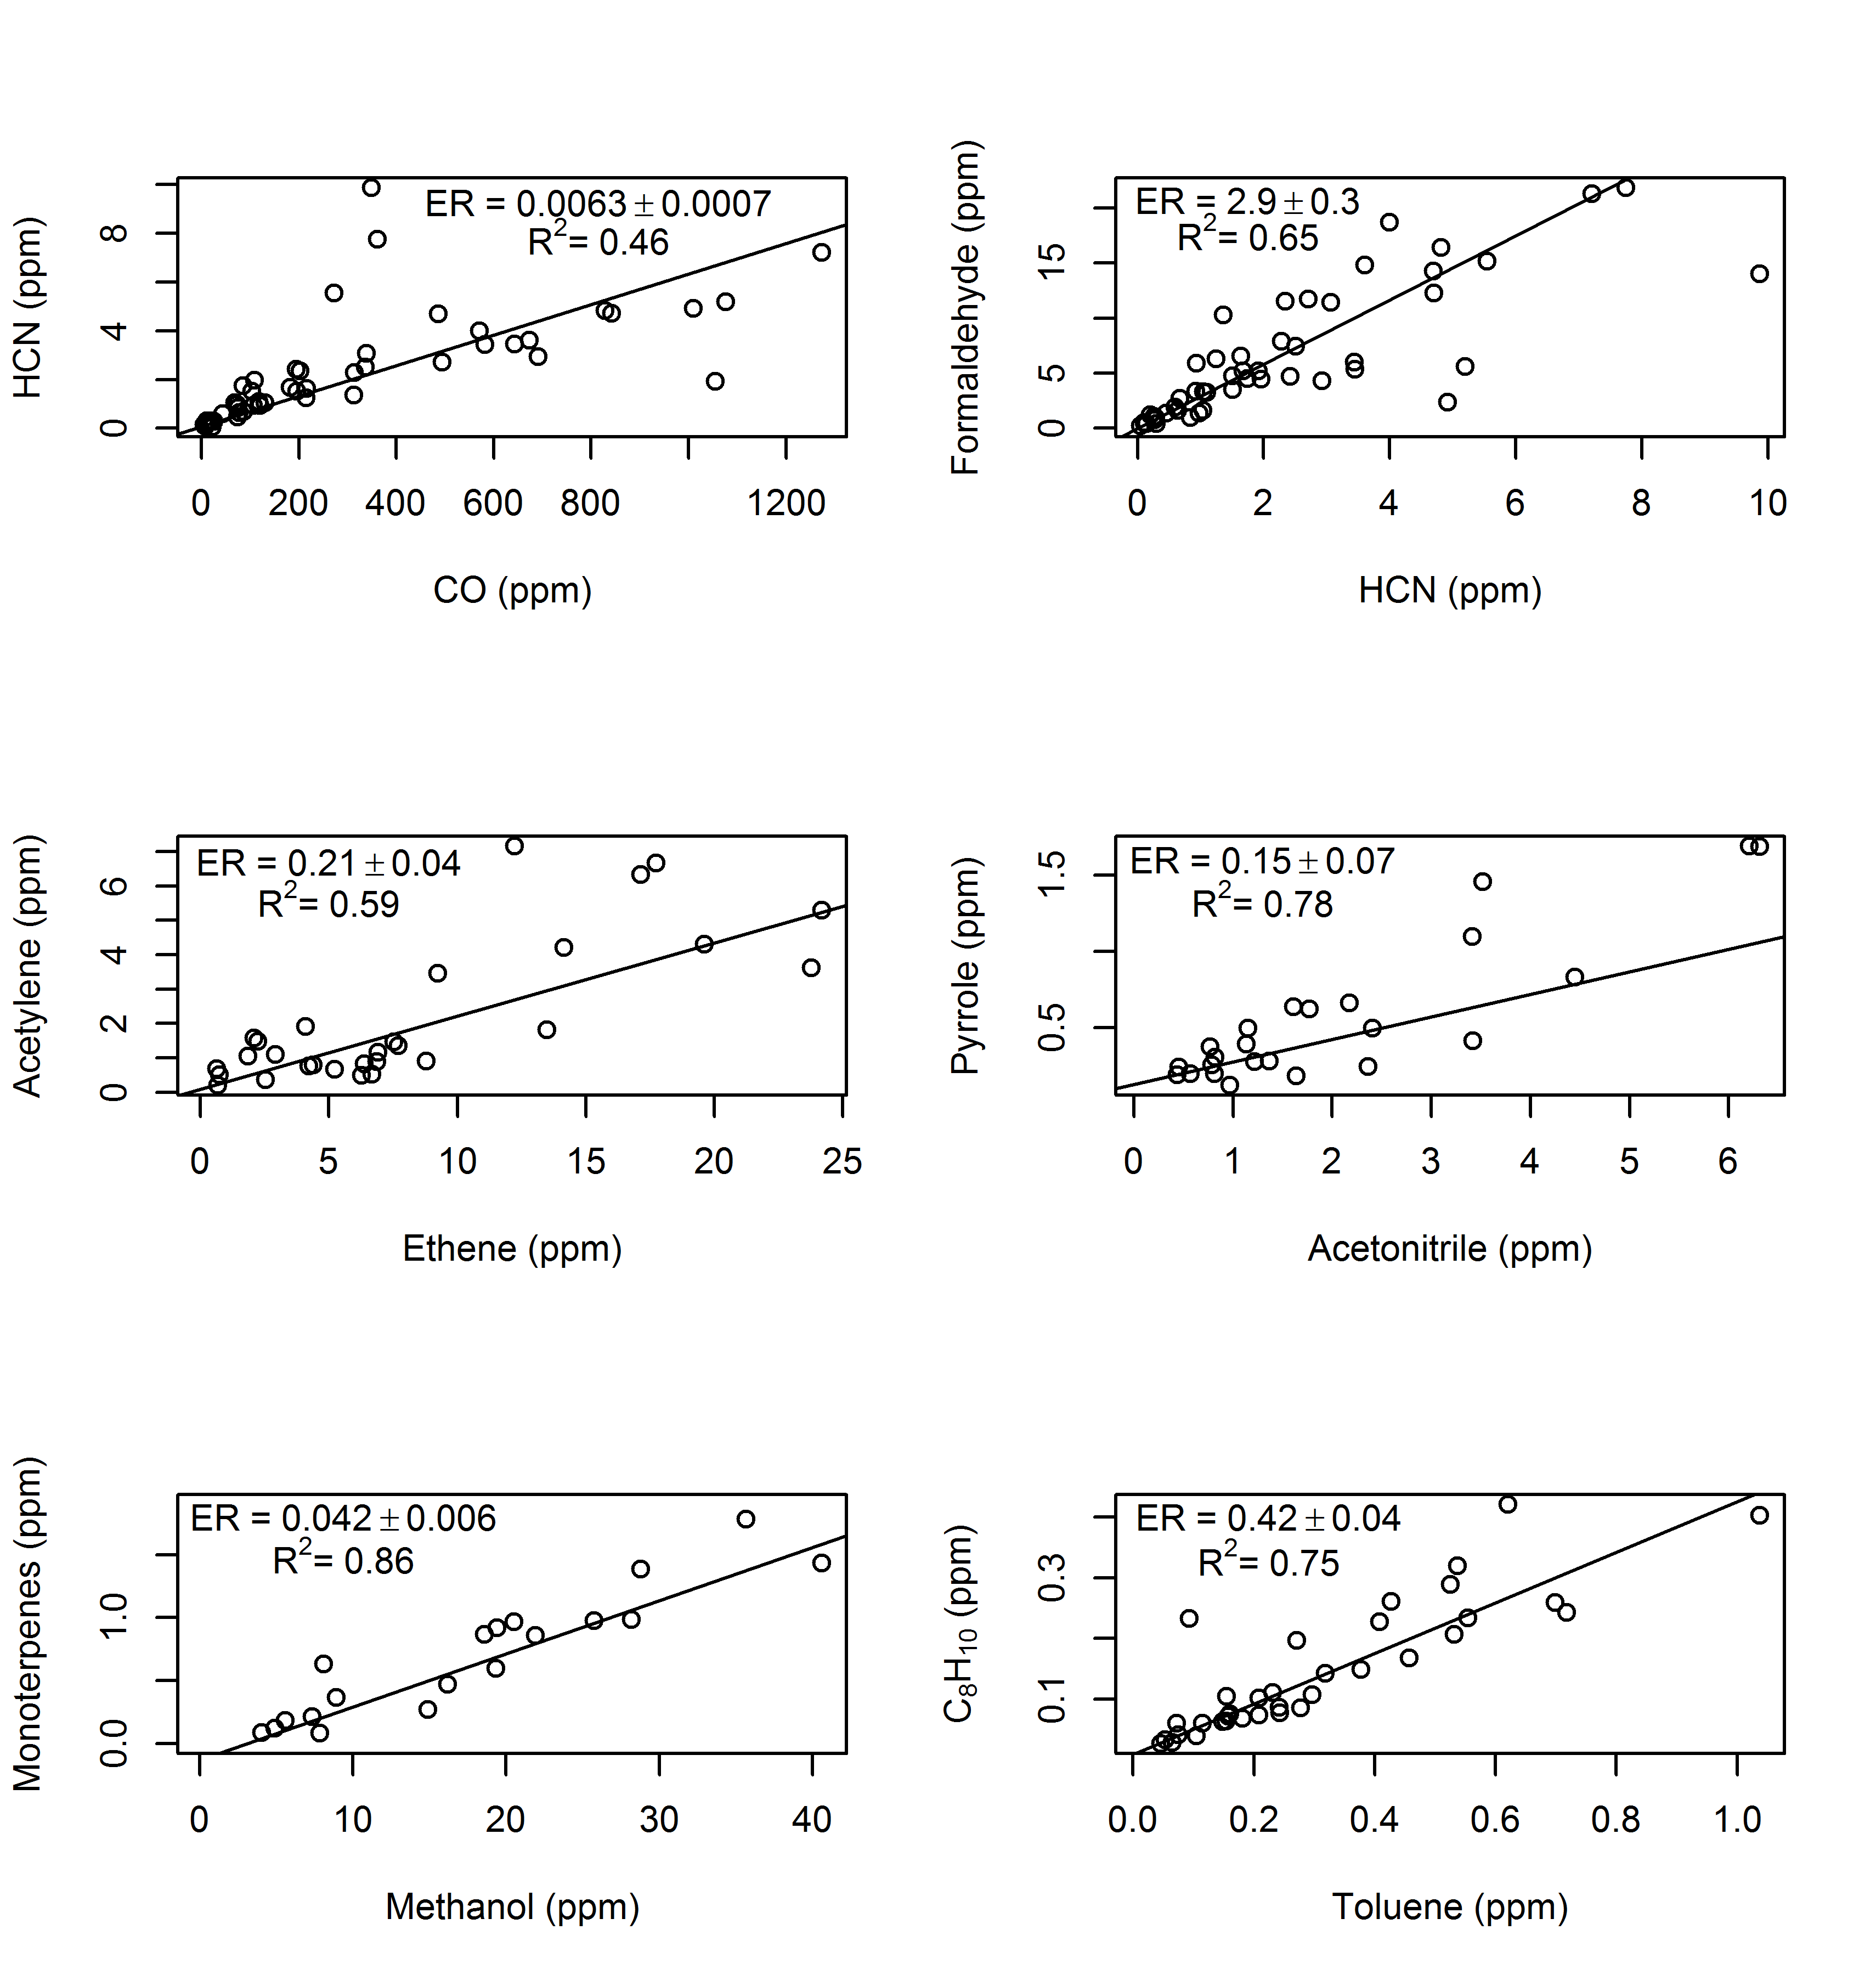
\includegraphics[width=14 cm]{C:/Users/eag873/Documents/GitHub/HRB_paper/supp/supp_figures/All_fires_examples.png}
  \caption{Examples of 'all data combined' correlations from the grab sample measurements. Top left is hydrogen cyanide (HCN) to CO, top right is formaldehyde to HCN, middle left is acetylene to ethene, middle right is pyrrole to acetonitrile, bottom left is monoterpenes to methanol and bottom right is the sum of C$_8$H$_{10}$ species to toluene.}
  \label{fig:all_data}
\end{figure}

Similarly, the emission ratio of acetonitrile to CO is markedly lower at Gulguer Plateau than at the other fires. This could be due to the lower nitrogen content of logs compared to foliage and twigs \citep{Susott1996,Snowdon2005}, resulting in lower emissions of nitrogen-containing species \citep{Coggon2016}. %The emission ratio measured for acetonitrile at Gulguer Plateau is excluded from the mean emission ratio listed in Table \ref{table:grab}. Including this emission ratio reduces the mean ER from 0.05 $\pm$ 0.01 to 0.04 $\pm$ 0.02. 
The Gulguer Plateau fire samples are excluded from the emission ratio for acetonitrile derived from combining data from all fires, since including them results in R$^2$ < 0.5. Figure \ref{fig:Acetonitrile} shows the correlations of acetonitrile with CO; the Gulguer Plateau fire is shown in red, the other four fires are shown in black. The emission ratio derived from the black line is not significantly different from the mean ER that includes the Gulguer Plateau data (see Table~\ref{table:grab}). 
Pyrrole showed the same behaviour against CO as acetonitrile. Its emission ratio was therefore derived to acetonitrile instead of CO.  

\begin{figure}
  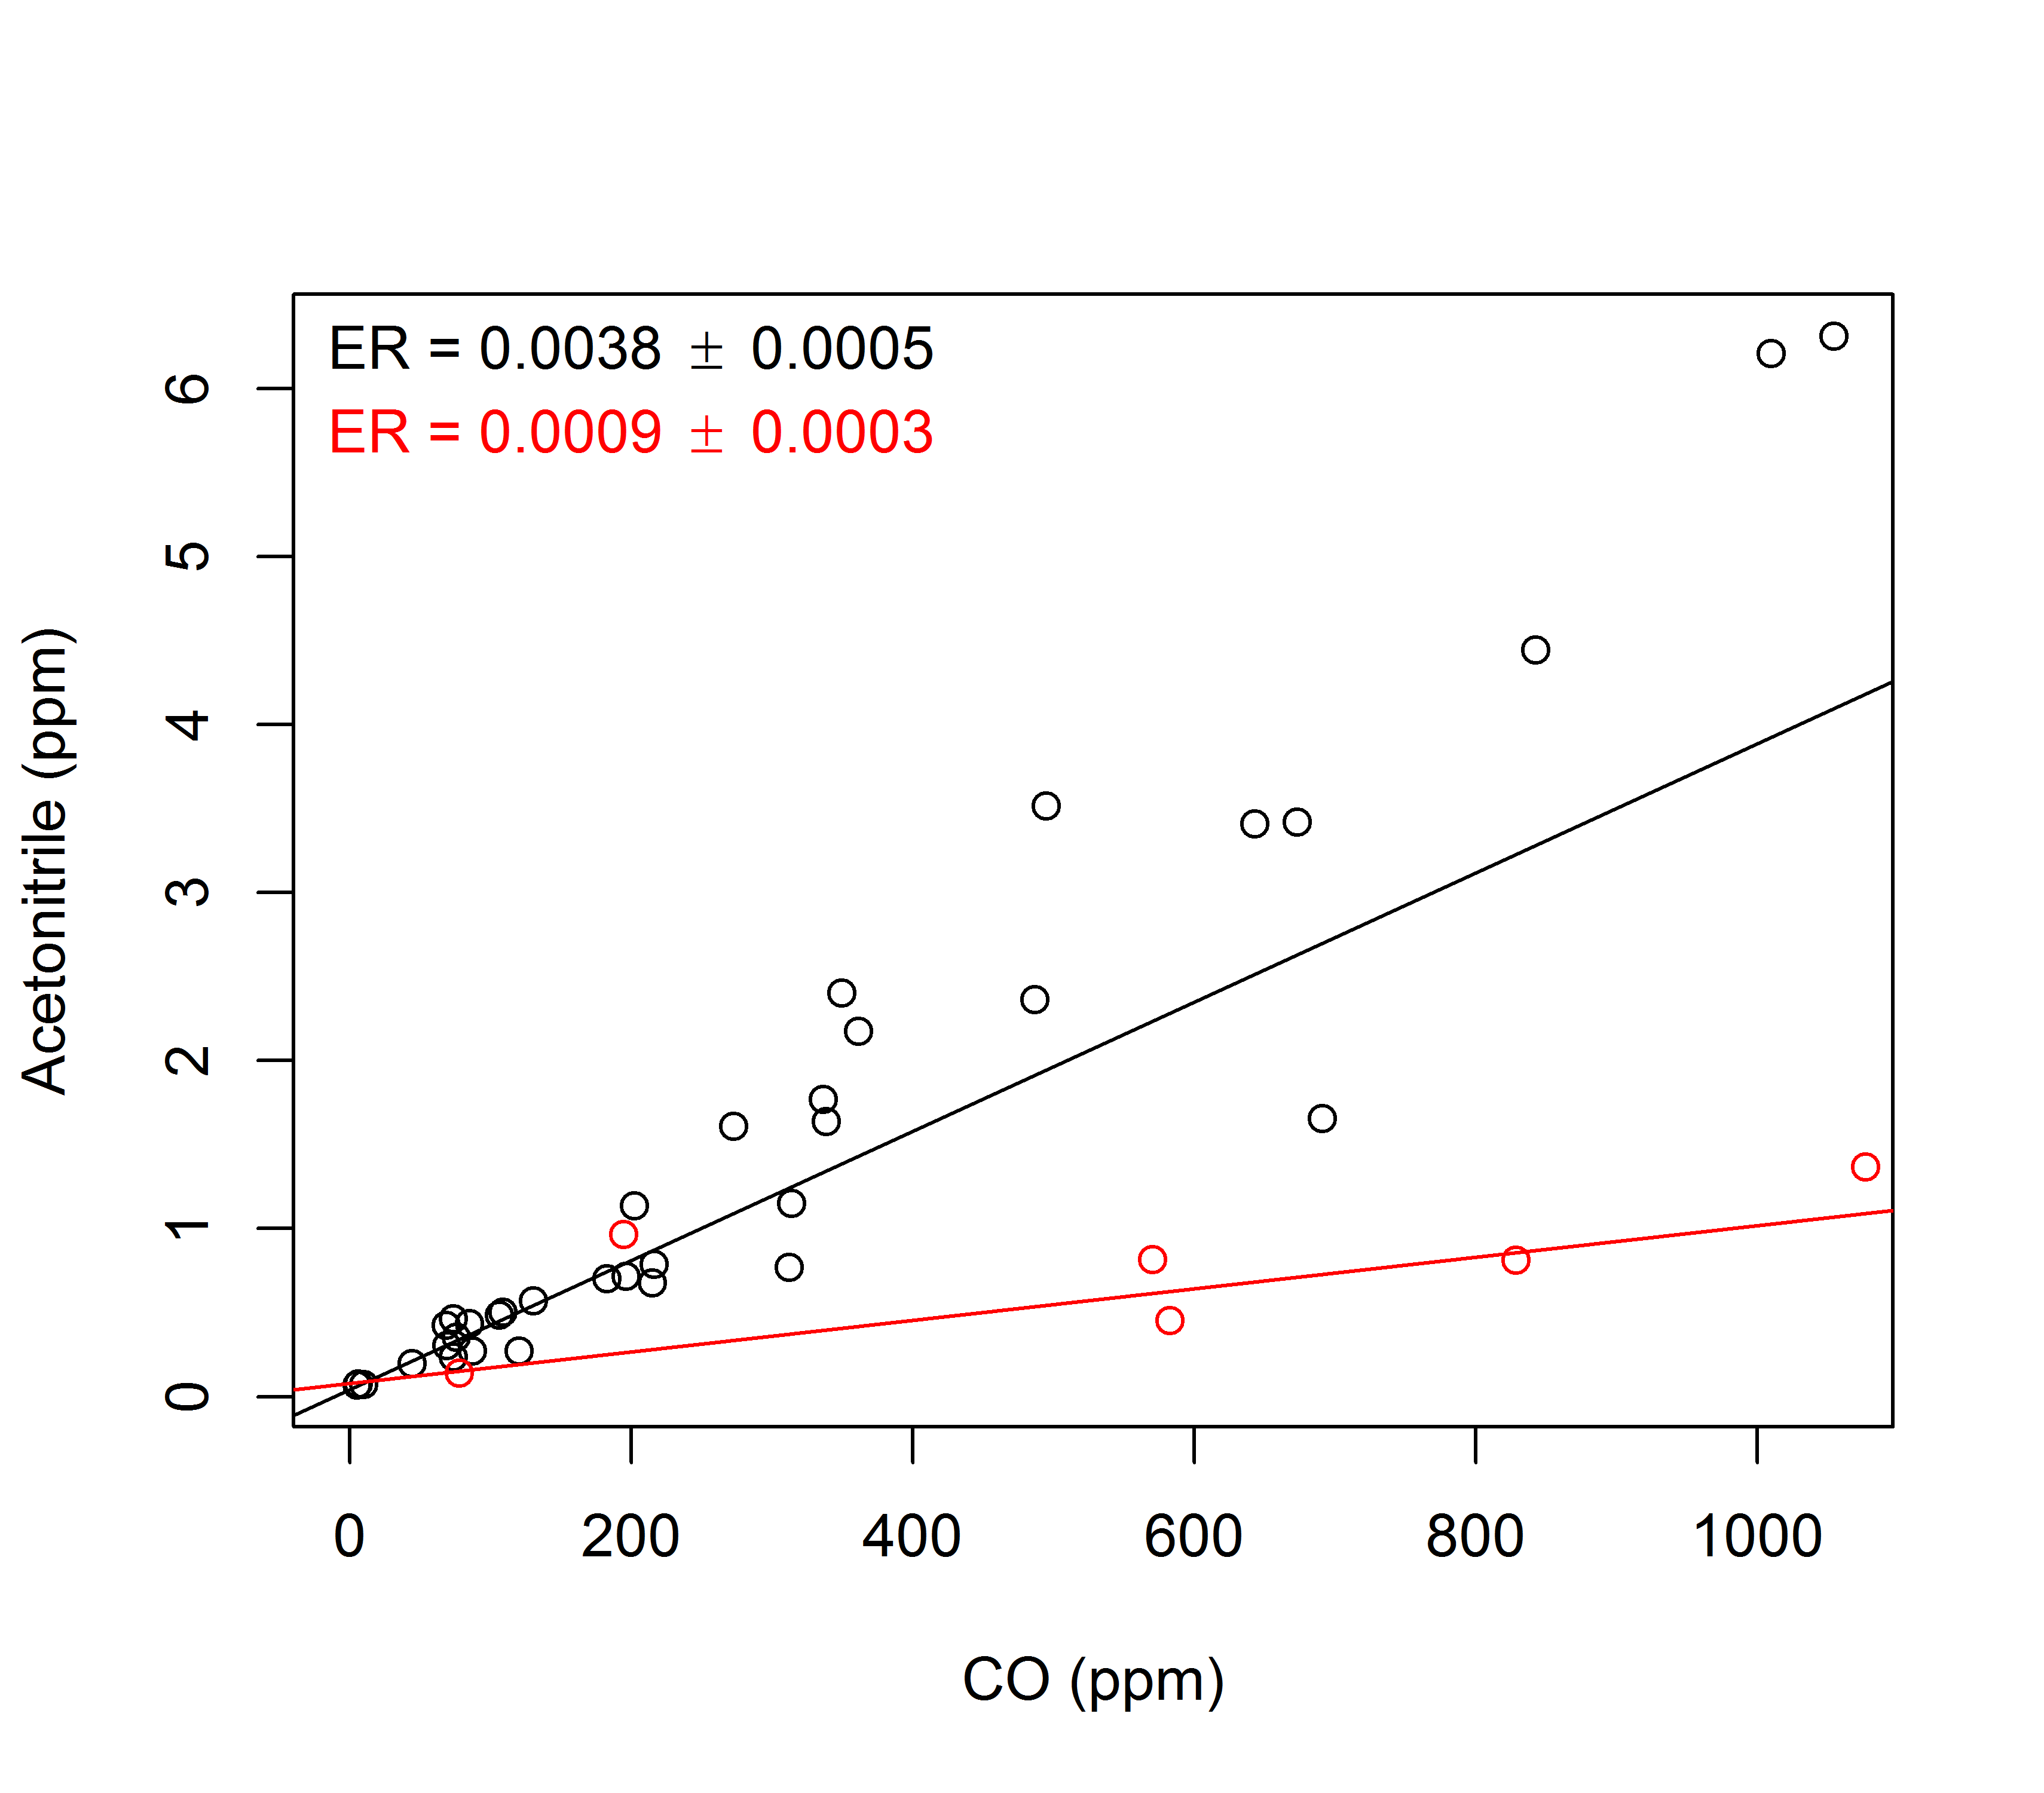
\includegraphics[width=8.3 cm]{C:/Users/eag873/Documents/GitHub/HRB_paper/figures/Acetonitrile.png}
  \caption{Emission ratio (ER) for acetonitrile to CO for the Gulguer Plateau fire grab samples (in red) and for the other four fires (in black).}
  \label{fig:Acetonitrile}
\end{figure}

Despite this site-to-site variability in the emission ratio of certain species, the mean emission ratio is usually the same, within the uncertainties, as the value derived from combining samples from all fires. 
This indicates that the 'all data combined' emission ratios listed in Table~\ref{table:grab} are representative of the ecosystem sampled - a useful result since this is the only ER available for some species. 
Whole-fire emission factors were then calculated using the 'all data combined' emission ratios listed in Table~\ref{table:grab} and the average fire-integrated emission factors for CO and CO$_2$ measured by OP-FTIR at the NSW fires by \citet{Paton-Walsh2014} and reproduced in the last column of Table~\ref{table:OP}. The resulting ecosystem-average emission factors for all VOC species are listed in Table \ref{table:comp}.  


\subsection{Open-path FTIR results from prescribed fires in temperate forests in Victoria }

\begin{table} 
  \caption{Summary of open-path FTIR measurements at prescribed fires in temperate forest in the State of Victoria and comparison with similar results obtained at prescribed fires in New South Wales. Values in parentheses are standard deviations of the mean.}
 \begin{tabular}{l l l l l l l l l l  } 
   \tophline
   & & Castlemaine & & & Greendale & & & NSW fires$^a$ & \\
   %&&&&&&&&\citep{Paton-Walsh2014}&\\
   Species & Reference &ER & R$^2$ & EF & ER & R$^2$ & EF &  ER & EF \\
   &species&&&&&&&&\\
   \hline
   CO$_2$ & & & & 1650 $\pm$ 170 & & & 1670 $\pm$ 170 & & 1620 (160) \\
   CO & & & & 101 $\pm$ 16 & & &84 $\pm$ 13 & & 118 (19) \\
   CH$_4$ & CO & 0.0571  $\pm$   & 0.97 & 3.3 $\pm$ 0.2 & 0.0633 $\pm$ & 0.99 & 3.1 $\pm$ 0.2 &  0.05  & 3.6 (1.1) \\
   & &0.0006& & & 0.0005 &  &&(0.01)&\\
   Ammonia & CO & 0.0276 $\pm$ & 0.98 & 1.7 $\pm$ 0.2 & 0.0291 $\pm$& 0.95 & 1.5 $\pm$ 0.2 & 0.021  & 1.6 (0.6)\\
    & &  0.0003& & & 0.0004 &  &&(0.008)&\\
   Ethene & CO$_2$ & 0.00118 $\pm$ & 0.97 & 1.2 $\pm$ 0.3 & 0.00105 $\pm$ & 0.91 & 1.1 $\pm$ 0.2 & 0
   .0012& 1.3 (0.3) \\
   & &  0.00001& & & 0.00002 &  &&(0.0003)&\\
   Formaldehyde & CO$_2$ & 0.00133 $\pm$ & 0.94 & 1.5 $\pm$ 0.3 & 0.00113 $\pm$& 0.82 & 1.3 $\pm$ 0.2 & 0.0016 & 1.7 (0.4) \\
   & &  0.00002& & & 0.00003 &  &&(0.0004)&\\
   Methanol & CO & 0.0144 $\pm$& 0.96 & 1.7 $\pm$0.3 & 0.0154 $\pm$& 0.95 & 1.5 $\pm$0.4 & 0.017 & 2.4 (1.2) \\
   & &  0.0002& & & 0.0006 &  &&(0.006)&\\
   Formic acid & CO & 0.00321 $\pm$& 0.94 & 0.5 $\pm$ 0.2 & 0.00414 $\pm$& 0.93 & 0.6 $\pm$ 0.1 & 0.0021 & 0.4 (0.2)\\
    & &  0.00005& & & 0.00007 &  &&(0.0007)&\\
   Acetic acid & CO & 0.0303 $\pm$ & 0.98 & 6.5 $\pm$ 1.2 & 0.0331 $\pm$& 0.95 & 6.0 $\pm$ 0.9 & 0.015 & 3.8 (1.3)\\
     & &  0.0003& & & 0.0005 &  &&(0.003)&\\
 \bottomhline
\end{tabular}
\label{table:OP}
  \belowtable{$^a$ \citet{Paton-Walsh2014}} % Table Footnotes
\end{table}

All trace gases measured by OP-FTIR at the prescribed fires in Victoria exhibited strong correlations with either CO or CO$_2$. Correlations between the measured species at the Castlemaine fire are shown in Figure S2 as an example. The calculated emission ratios and emission factors are listed in Table~\ref{table:OP}. %Uncertainties were calculated as per Appendix B of \citet{Paton-Walsh2014}. 

There is little variability seen between the two fires sampled in Victoria. The emission ratios measured at the two fires are comparable, and the emission factors agree within their uncertainties. The emission ratios measured in Victoria are within the range of values measured at the NSW fires for all species except formic acid and acetic acid (Table \ref{table:OP}).  
The average observed MCE of 0.92 at the Victorian fires is higher than that reported by \citet{Paton-Walsh2014} for the NSW fires (average 0.90, range: 0.88-0.91). The emission factors listed in Table \ref{table:OP} generally reflect this difference, with species typically associated with smouldering combustion having slightly lower emission factors at the Victorian fires. The differences are slight however, and the emission factors from Victoria agree within the uncertainties with those from NSW. One major exception is acetic acid. Its emission ratio at the fires in Victoria was double that seen at the NSW fires, and this is reflected in the emission factors. This indicates a difference in emissions from the different regions sampled that is not explained by the difference in modified combustion efficiency. The dependence of emission factors derived from the OP-FTIR measurements on MCE is explored more fully in the next section.  


\subsection{Dependence of emission factors of trace gases from Australian temperate forest fires on modified combustion efficiency (MCE)}

The MCE dependence of the emissions of carbon-containing species from all fires sampled using OP-FTIR as part of this ground-based study is explored in this section. The emission factors calculated for each fire sampled by OP-FTIR are plotted as a function of MCE in Fig.~\ref{fig:MCE_dep}. The regression statistics are listed in Table~\ref{table:MCE_dep}. As the range of observed MCE is relatively narrow, the relationship is well represented using a linear regression. For larger MCE ranges, an exponential fit may be more appropriate (e.g. \citet{Meyer2012} suggest an exponential fit for CH$_4$). 

The magnitude of the slope and the intercept listed in Table~\ref{table:MCE_dep} reflects the magnitude of the emission factor for that species. The strength of the relationship is judged from the coefficient of determination (R$^2$) and the p-value (the probability that there is no correlation between x and y). A poor R$^2$ indicates that MCE alone cannot explain the variability in EF. 

\begin{figure}
  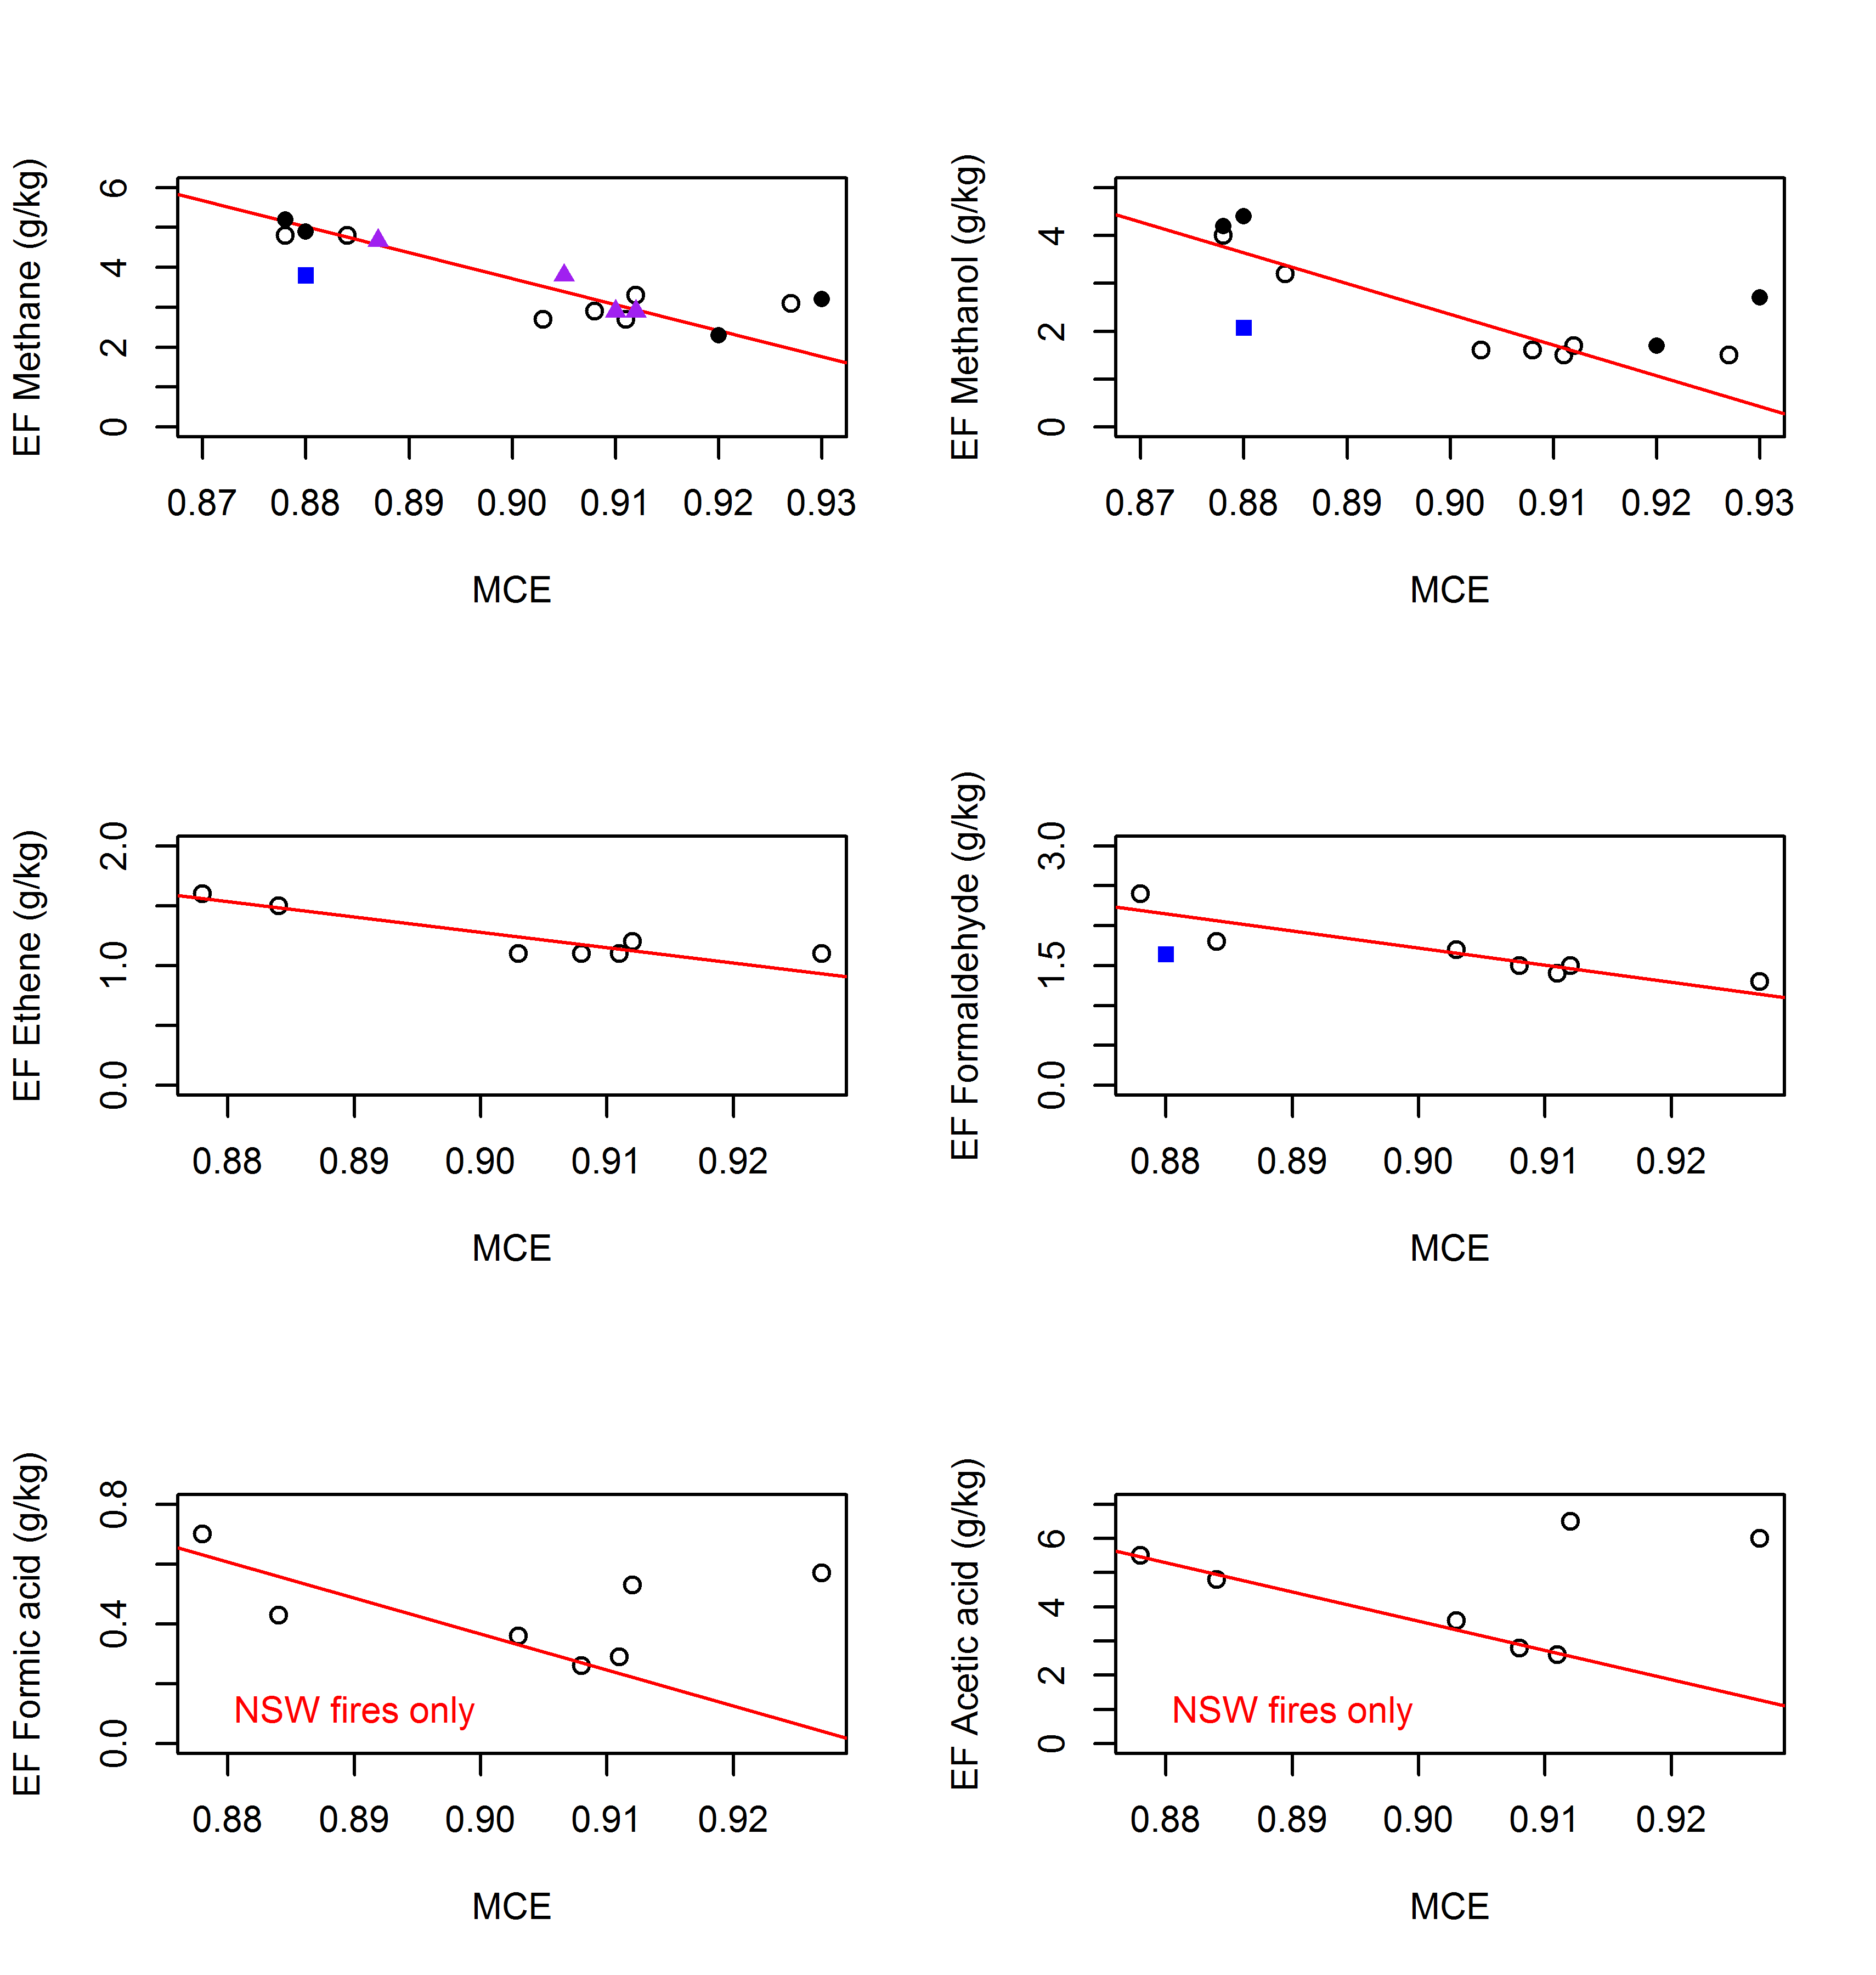
\includegraphics[width=12 cm]{C:/Users/eag873/Documents/GitHub/HRB_paper/figures/MCE_v3.png}
  \caption{Dependence of emission factors on MCE. Open circles represent the seven fires sampled using OP-FTIR with the line of best fit shown in red. For formic acid and acetic acid, this regression line was derived using the measurements from the NSW fires only. The black circles represent average results from grab samples at four fires (The grab sampling results from the Gulguer Plateau fire are either not available (methanol) or fall outside the range measured by OP-FTIR (methane) and therefore do not appear). The purple triangles represent the methane results from the airborne measurements of Hurst et al. (1996) and the blue squares represent the emission factors measured for methane, methanol, and formaldehyde by Lawson et al. (2015) in a transported plume impacting the Cape Grim Baseline Air Pollution Station in Tasmania.
  }
  \label{fig:MCE_dep}
\end{figure}

\begin{table}
    \caption{Summary of regression statistics for the emission factor dependence on modified combustion efficiency (MCE) of carbon-containing species measured by open-path FTIR in temperate forest fires in Australia}
  \begin{tabular}{l l l l l l } 
    \tophline
   Species & Data used in &  Slope & Intercept & R$^2$ & p value \\
   & regression calculation &&& &\\
   \hline
  CH$_4$& NSW and VIC fires & -65 $\pm$ 20 & 62 $\pm$ 17 & 0.61& 0.02 \\ 
  Ethene & NSW and VIC fires& -13 $\pm$ 4 & 13 $\pm$ 3 & 0.75 & 0.007 \\
  Formadehyde & NSW and VIC fires& -21 $\pm$ 10& 21 $\pm$ 9& 0.79 & 0.005\\
  Methanol  & NSW and VIC fires& -64 $\pm$ 16 & 60 $\pm$ 14 & 0.79 & 0.005\\
  Formic acid  & NSW fires only & -12 $\pm$ 6& 11 $\pm$ 5 & 0.74 & 0.04\\ 
  Acetic acid  & NSW fires only & -86 $\pm$ 5 & 81 $\pm$ 4 & 0.98 & 0.004 \\ 
  sum of furan and isoprene & Grab samples & -9 $\pm$ 5 & 9 $\pm$ 4 & 0.95 & 0.005 \\ 
  sum of acetone and propanal & Grab samples & -5 $\pm$ 2& 6 $\pm$ 1& 0.94 & 0.009 \\ 
    \bottomhline
  \end{tabular}
  \label{table:MCE_dep}
  \belowtable{} % Table Footnotes
\end{table}

For some species, there is no significant relationship with MCE when including data from all seven fires. This is the case for formic acid and acetic acid, for which significantly different emission ratios were measured at the fires in Victoria. Similarly, the emission factor for CH$_4$ has a stronger relationship with MCE when considering only the NSW fires. This indicates that combustion efficiency is not the only factor that controls differences in emissions for these species. 

For comparison purposes, the emission factors measured by \citet{Hurst1996} for CH$_4$ and \citet{Lawson2015} for CH$_4$, methanol and formaldehyde are also plotted in Fig.~\ref{fig:MCE_dep}. Figure~\ref{fig:MCE_dep} also shows the average results derived for CH$_4$ and methanol from the grab samples. The grab sampling results from the Gulguer Plateau fire are either not available (methanol) or fall outside the range measured by OP-FTIR (methane) and therefore do not appear in Fig.~\ref{fig:MCE_dep}. 
%The reasonable agreement between the grab sampling results and the OP-FTIR measurements seen in Fig.~\ref{fig:MCE_dep} means that it may be possible to estimate the
The MCE-dependence of the species that were only measured in the grab samples (by SIFT-MS or White-cell FTIR) was also tested. For this analysis, average values from the five fires were used, spanning a range of average MCE of 0.78 to 0.93. No statistically significant trend was found for acetaldehyde, acetonitrile, benzene, butadiene, ethane and toluene, but there were significant trends for the sum of furan and isoprene and for the sum of acetone and propanal. The statistics for these trends are listed in Table~\ref{table:MCE_dep}. The MCE dependence of the other measured species could not be determined because fire-specific emission ratios were not available. 

\section{Discussion}

\subsection{Comparison with MCE-dependent emission factors from North American temperate forests}

The MCE dependence of emission factors listed in Table \ref{table:MCE_dep} were compared to those reported by \citet{Akagi2013} for fires in conifer forests in South Carolina, and by \citet{Burling2011} for fires in conifer forests in North Carolina and for chaparral fires in California. There is considerable variability between the two North American studies, even for the similar conifer ecosystems sampled. 
Both studies found negative relationships to MCE for CH$_4$ (with slopes ranging from -65 $\pm$ 13 to -96 $\pm$ 10), methanol (with slopes ranging from -21 $\pm$ 6 to -39 $\pm$ 2) and furan (-6 $\pm$ 3 to -8 $\pm$ 1). These results are consistent with the ones listed in Table~\ref{table:MCE_dep} for these species, although the slope measured in Australian temperate forests for methanol is larger (-64 $\pm$ 16). 

For other species, the results are mixed, with \citet{Akagi2013} finding no relationship to MCE for acetic acid but \citet{Burling2011} finding a strong one (with a slope of -45 $\pm$ 3 and R$^2$ = 0.98) in a similar conifer ecosystem. This is analogous to the results presented here, where a strong relationship to MCE is found for a subset of the data (NSW fires only, slope = -86 $\pm$ 5, R$^2$ = 0.98) but no relationship is found when all the fires are considered. 
For formic acid, both North American studies find a relationship for conifer forest fires (with slopes of -1.8 $\pm$ 0.6 and -3.1 $\pm$ 0.2), but \citet{Burling2011} found no relationship for chaparral fires. In this study, we find a relationship for the NSW fires, but no relationship when including all fires. 

For formaldehyde and ethene, \citet{Akagi2013} reports a weak or insignificant relationship to MCE whereas \citet{Burling2011} reports strong relationships to MCE for both species for fires in a similar conifer ecosystem (with slopes of -21 $\pm$ 2 for formaldehyde and -11 $\pm$ 2 for ethene) and a weak or insignificant relationship to MCE for fires in chaparral. For fires in Australian temperate forests, we observed similar slopes of -21 $\pm$ 10 for formaldehyde and -13 $\pm$ 4 for ethene. 

\citet{Akagi2013} report a slope of -16 $\pm$ 4 for acetone, which is larger than the one observed for the sum of acetone and propanal in this study (-5 $\pm$ 2). \citet{Akagi2013} also report significant relationships to MCE for ethane, benzene, toluene, xylenes, acetonitrile and acetaldehyde whereas no relationship was observed for these species in our study.
   
Considering the variability of relationships to MCE observed even for similar ecosystems, it seems likely that other factors are influencing emissions. %, especially of those species that are biogenically produced by vegetation and are not only a product of combustion.
\citet{Burling2011} sampled spring fires whereas \citet{Akagi2013} sampled autumn fires so it is possible that some of the variability is due to seasonal differences. In this study, fires were sampled over several years, both in spring (August-September) and in autumn (April-May). There is no obvious seasonal effect in the data, however there seems to be regional effects, especially for formic acid and acetic acid, and these may be due to differences in vegetation.   
This variability limits the usefulness of MCE as a means of extrapolating emission factors for these species. Nevertheless, the MCE measured at a fire can be a good indication of whether a representative sample has been captured. This is explored in the next section by comparing MCE values observed from different measurement platforms for Australian temperate forest fires. 

\subsection{Comparison of MCE, CO$_2$, CO and CH$_4$ emission factors measured for Australian temperate ecosystems from various platforms}


\begin{table}
 \caption{Comparison of whole-fire modified combustion efficiency (MCE) and whole-fire emission factors for CO$_2$, CO and CH$_4$ reported in the literature for fires in Australian temperate forests and temperate forests in North America.}
 \begin{tabular}{l l l l l l l l } 
   \tophline
   Study & Location & MCE & EF CO$_2$ & EF CO & EF CH$_4$ & Platform & Type of fire \\ 
   \hline
   \citet{Hurst1996}$^a$ & Helensburgh, NSW, & 0.91 & 1577 & 99&2.9 & Airborne & Wildfire\\
   &Australia &&&&&&\\ 
   & Worragee, NSW,& 0.89 & 1540 & 125 & 4.7 & Airborne & Wildfire \\
   &Australia &&&&&&\\ 
   & Sydney, NSW, & 0.91 & 1558 & 104 & 3.8 & Airborne & Wildfire \\
   & Australia &&&&&&\\ 
   & Bateman's Bay, NSW,& 0.91 & 1577 & 97 &2.9 & Airborne & Prescribed  \\
   & Australia &&&&&& fire\\ 
  % & & & & & &  &  \\
  \citet{Lawson2015} & Robbin Island, TAS, & 0.88 & 1621 & 127 &3.8 & Transported  & Wildfire \\
  & Australia & & & & & plume & \\
  \citet{Paton-Walsh2014} & Greater Sydney Area, & 0.90 (0.2) & 1620 (160) & 118 (19) & 36 (1.1) & Ground-based  & Prescribed \\
      &  NSW, Australia& & & & & OP-FTIR& fires \\
   \citet{Rea2016} & Greater Sydney Area, & 0.91 & 1640& 107& 7.8$^b$& Transported  & Wildfires \\
     & NSW, Australia& & & & & plume& \\   
   This study & Central Highlands, VIC, & 0.92 (0.01) & 1660 (170) & 93 (15) & 3.2 (0.2) & Ground-based & Prescribed  \\
     &Australia & & & & & OP-FTIR & fires\\
   \citet{Akagi2011}$^c$ & North America & $\sim$0.92 & 1647 (37) & 88 (19) & 3.4 (0.9) & Mixed & Prescribed \\ 
  & & & & & & &  $\&$ wild fires \\ 
 \bottomhline
 \end{tabular}
\belowtable{
$^a$ \citet{Hurst1996} assume 6 $\%$ of carbon is emitted as ash, which explains the lower emission factors reported for CO$_2$

$^b$ this value may be influenced by other sources - see \citet{Rea2016}

$^c$ Table S4, February 2015 update. MCE estimated from reported emission factors for CO$_2$ and CO. 
} % Table Footnotes
 \label{table:MCE_comp}
\end{table}


MCE and emission factors for CO$_2$, CO and CH$_4$ for Australian temperate ecosystems have been measured from a variety of platforms, including airborne measurements \citep{Hurst1996} and measurements of plumes transported short distances to fixed monitoring stations \citep{Lawson2015,Rea2016}. Comparing these results to our ground-based measurements (see Table~\ref{table:MCE_comp}) reveals that there is a relatively small spread of MCE values measured for fires in Australian temperate ecosystems. %Even airborne measurements over the very large Sydney wildfires of January 1994 have a relatively low average MCE of 0.91 \citep{Hurst1996}. Furthermore,
 There is no significant difference in the MCE observed for wild or prescribed fires, or between measurement platforms (Kruskal-Wallis rank sum test, p > 0.7). This is in contrast with measurements conducted at prescribed fires in North America, where higher average MCE values were observed for airborne measurements than for open-path measurements on the ground (0.93 vs. 0.91 on average for the same fires in \citet{Akagi2014}, for example). MCE values of 0.93 or greater for airborne measurements have also been reported by other US studies \citep{Burling2011, Akagi2013}. The top left panel of Fig.~\ref{fig:MCE_dep} shows the CH$_4$ emission factors reported by \citet{Hurst1996} plotted alongside the OP-FTIR measurements conducted as part of this study and as part of \citet{Paton-Walsh2014}. The agreement between the two platforms is excellent. 
The good agreement for MCE between platforms and fire type could be coincidental, or an artefact of the sampling approaches, or may in fact indicate that the prescribed and wild fires sampled burnt at a similar MCE.  \citet{Liu2017}, studying wildfires in the western US, report EF for PM that are a factor of two higher for wildfires than for prescribed fires burning at the same MCE, but do not observe the same for trace gases such as CH$_4$.  
 No PM data are available from the studies listed in Table~\ref{table:MCE_comp}, but CH$_4$ data are. The average emission factor measured for CH$_4$ in Australian temperate forests is 3.5 (0.8) g kg$^{-1}$ dry fuel burnt (this value excludes the emission factor reported by \citet{Rea2016} as it may have been influenced by other sources). The average for the ground-based OP-FTIR measurements is 3.5 (0.9) g kg$^{-1}$ dry fuel burnt. These are in excellent agreement with the emission factor for CH$_4$  of 3.4 (0.9) g kg$^{-1}$ dry fuel burnt listed for temperate forests in \citet[Table S4, February 2015 update]{Akagi2011}. 

\subsection{Comparison of VOC emission ratios and emission factors measured for temperate ecosystems}
Measurements of VOC emission factors have been more limited for Australian temperate forests. Enhancement ratios to CO for methanol, ammonia, formic acid, formaldehyde, acetylene, ethene and ethane were measured in lofted plumes from wildfires by ground-based solar remote sensing Fourier transform spectrometry \citep{Paton-Walsh2005, Paton-Walsh2008} and satellite-based spectroscopic measurements \citep{Young2011,Glatthor2013}. These were compared to the emission ratios measured in fresh smoke by OP-FTIR in NSW by \citet{Paton-Walsh2014}. They found good agreement for methanol and formaldehyde, and evidence for depletion of ammonia and ethene and formation of formic acid in aged smoke. 
 
The only other study to have reported emission factors for a significant number of trace gas species is that of \citet{Lawson2015}. They report emission ratios and emission factors for trace gases and aerosol from opportunistic measurement of a biomass burning plume impacting Cape Grim Baseline Air Pollution Station in Tasmania in February 2006. The plume was advected to the Station from a fire in coastal heath on a nearby island, mostly at night (from 23:00 AEST until 09:00 AEST). The vegetation burnt in the Robbins Island fire is similar to what typically burns in a prescribed fire, so their emission ratios and emission factors for VOCs are listed alongside ours in Table~\ref{table:comp}. Emission factors from  \citet[Table S4, February 2015 update]{Akagi2011} are also included for comparison. For some of the species measured by SIFT-MS in this study and by PTR-MS in \citet{Lawson2015}, the reported emission factors are sum measurements of several species, including potential contributions from unidentified compounds. In these cases, the emission factors of all species that could contribute were sourced from \citet[Table S4, February 2015 update]{Akagi2011} and listed in the last column of Table~\ref{table:comp}. 

There is considerable variability in the emission factors listed in Table~\ref{table:comp}, and most species agree within their stated uncertainties. Nevertheless, comparing average values highlights potential differences between emissions from Australian temperate forests and emissions from North American temperate forests. Emission  factors for both hydrogen cyanide and ethene are in excellent agreement, and emission factors for methanol, formaldehyde and 1,3-butadiene are within 20$\%$ of each other. Emission factors for ethane, acetylene and toluene also agree quite well, being within about 30$\%$ of each other. However, Australian forest fires potentially emit 50$\%$ more formic acid, twice as much acetic acid and ammonia, less than half as much ethanol and monoterpenes, and two to ten times more acetonitrile and pyrrole than North American fires. 

Nitrogen-containing VOCs make little contribution to the overall reactivity of a smoke plume \citep{Gilman2015}. Acetonitrile has an atmospheric lifetime on the order of months and is a tracer for long-range transport of biomass plumes \citep{Bange2000}, whereas more reactive nitrogen-containing species may be tracers for fresh plumes \citep{Gilman2015,Coggon2016}. Higher emissions may affect estimates of plume age based on these species. 
The difference with the North American fires may be due to higher fuel nitrogen content. Acacia are nitrogen-fixing species that have high leaf N content (1.50-3.55$\%$) which is partly conserved through leaf fall, leading to higher nitrogen in the leaf litter \citep{Snowdon2005}. Acacia are some of the dominant understorey species in the forests investigated in this study, and their presence may have contributed to the high emissions of nitrogen-containing species; however, without fuel composition measurements, it is impossible to draw definitive conclusions. 

%Lower emissions of compounds such as monoterpenes would impact downwind plume chemistry as the smoke is photochemically processed (Akagi et al. 2013).
The initial mixture of trace gases emitted by a fire is one of the factors (along with meteorology and the presence of other sources) that influences plume aging \citep{Akagi2012,Jaffe2012} and air quality outcomes downwind of the fires.  
The use of Australian-specific emission factors is therefore recommended in studies looking at the regional impact of fires in Australian temperate forests. 


 \tablecaption{Comparison of VOC emission ratios and emission factors reported in the literature for fires in temperate forests in Australia and in North America. Emission ratios (ER) are in mol mol$^{-1}$ and emission factors (EF) are in g kg$^{-1}$ dry fuel burnt. Unidentified species that are likely to contribute to the signal measured by SIFT-MS are listed by their molar mass in the last column.}
  \tablehead{
  \hline
   &\multicolumn{6}{c}{This study}&\multicolumn{3}{c}{References} \\
  &\multicolumn{4}{c}{White cell FTIR and SIFT-MS analysis of grab samples}&\multicolumn{2}{c}{Open-path FTIR}&\multicolumn{2}{c}{Lawson et al.}&Akagi et al. \\
  &\multicolumn{4}{c}{- prescribed fires in NSW}&\multicolumn{2}{c}{- average values}&\multicolumn{2}{c}{2015}&2011 \\
  Species & MM & ref.  & ER & EF &ER &EF &ER &EF & EF   \\
  %& &species & & & & & & & \\temperate  \\
  %&  & & & & & & & & forests \\
  \hline}
% \tablelasttail{$^a$ includes benzaldehyde}
\begin{supertabular}{l l l r l r l l l c}
    Ammonia & 17 &  CO & & & 0.023  & 1.6 (0.6) & & & 0.8 (0.4) \\
     &  & & & & (0.007)& & & & \\
  Acetylene & 26  & CO$_2$ & 0.00037  & 0.35 $\pm$ 0.09 & & & & & 0.26 (0.04) \\ 
  &&&$\pm$ 0.00008&&&&&&\\
  Hydrogen  & 27 & CO & 0.0063  & 0.7 $\pm$ 0.2 & & & 0.0057 & 0.7 & 0.7 (0.2) \\ 
  cyanide&&&$\pm$ 0.0007&&&&&&\\
  Ethene & 28 &  CO & 0.009 & 1.1 $\pm$ 0.2& 0.011  & 1.2 (0.2) & & & 1.2 (0.2) \\ 
  &&&$\pm$ 0.001&&(0.003)&&&&\\
  Ethane & 30  & CO & 0.0038 & 0.48 $\pm$ 0.09 & 0.004  & 0.5 (0.2) & 0.0032& 0.41 & 0.6 (0.2) \\
  &&&$\pm$ 0.0003&&(0.001)&&&&\\
  Formaldehyde & 30  & CO & 0.018 & 2.3 $\pm$ 0.5 &  & 1.7 (0.4) & 0.011 & 1.6 & 2.1 (0.4) \\
  &&&$\pm$ 0.003&&&&&&\\
  Methanol & 32  & CO & 0.022 & 3.0 $\pm$ 0.5 & 0.016  & 2 (1) & 0.014 & 2.1 & 1.7 (0.5) \\ 
  &&&$\pm$ 0.002&&(0.005)&&&&\\
  Acetonitrile & 41  & CO & 0.0038 & 0.7 $\pm$ 0.1 & & & 0.0013 & 0.25 & 0.12 (0.05) \\ 
  &&&$\pm$ 0.0005&&&&&&\\
  Acetaldehyde & 44  & CO & 0.007 & 1.3 $\pm$ 0.3& & &0.0044 &0.92 & 0.8 (0.2) \\
  &&&$\pm$ 0.001&&&&&&\\
  Ethanol & 46 & CO & 0.00021& 0.04 $\pm$ 0.01 & & & & & 0.10 (0.05) \\
  Formic acid & 46  &CO & && 0.003 & 0.45 (0.16) & & & 0.29 (0.09) \\ 
  &&&&&(0.001)&&&&\\
  Butadiene &54 & CO$_2$ & 0.000074 & 0.23 $\pm$ 0.04& & & & & 0.19 (0.05) \\ 
  &&&$\pm$ 0.000009&&&&&&\\
  sum of acetone  & 58 & CO & 0.0034 & 0.8 $\pm$ 0.2 & & & 0.002 &0.54 & 0.54 (0.15)  \\
  and propanal &&&$\pm$ 0.0005&&&&&& (acetone) \\
  & &  & & & & & & & 0.11 (0.05) \\
  & &  & & & & & & & (propanal)\\ [20mm]
  Acetic acid & 60  &CO & & & 0.020 & 4.5 (1.6) & & & 2.1 (0.7) \\
  &&&&&(0.009)&&&&\\ 
  Pyrrole & 67 & CO & 0.0006 & 0.16 $\pm$ 0.08 & & & && 0.012 (0.009) \\
  &&&$\pm$ 0.0003&&&&&&(pyrrole) \\
  & & & & & & & & & 0.047 (0.026) (MM67)\\
 % & &  & & & & & & & (MM67)\\
  sum of furan  & 68  & CO & 0.0019 & 0.5 $\pm$ 0.1 & & & 0.0053 & 1.7 & 0.3 (0.1)  \\ 
  and isoprene &&&$\pm$ 0.0003&&&&&& (furan)\\ 
  & &  & & &&&&&0.10(0.004) \\
  & &  & & &&&&&(isoprene)\\
  &&&&&&&&& 0.18 (0.08) (MM68) \\
%  &&&&&&&&& (MM68)\\
  sum of MACR,   & 70 &CO & 0.0035 & 1.0 $\pm$ 0.3 & & & 0.0012 & 0.38 & 0.05 (0.02)  \\ 
  MVK and  & &  & $\pm$ 0.0009 & && & & & (methacrolein)) \\
  2-butenal&&&&&&&&&0.16 (0.04) \\
  &&&&&&&&& (methyl vinyl ketone) \\
  &&&&&&&&& 0.2 (0.1) \\
  &&&&&&&&& (2-butenal)\\
  &&&&&&&&& 0.3 (0.2) (MM70) \\
%  &&&&&&&&& (? MM70) \\
  Butanone & 72 & CO & 0.00082 & 0.25 $\pm$ 0.05& & & 0.001 & 0.35 & 0.13 (0.04)  \\ 
  &&&$\pm$ 0.00007&&&&&& (butanone) \\
  &&&&&&&&&0.09 (0.04) (MM72) \\
%  &&&&&&&&&(MM72)\\
  Benzene & 78 &CO$_2$ & 0.00014 & 0.39 $\pm$ 0.07 & & & & 0.69 & 0.3 (0.1) \\
  &&&$\pm$ 0.00002&&&&&&\\
  Toluene & 92 & CO & 0.0006 & 0.23 $\pm$ 0.05 & & &0.00069 &0.30 & 0.19 (0.05) \\ 
  &&&$\pm$ 0.0001&&&&&&\\
  sum of C$_8$H$_{10}$  & 106 & CO & 0.00025 & 0.11 $\pm$ 0.03 & & & 0.00053 & 0.26 & 0.17 (0.14)  \\
  species &&&$\pm$ 0.00005&&&&&  & (C$_8$ aromatics) \\
  &&&&&&&& &0.2 (0.1) \\
  &&&&&&&&&(benzaldehyde)\\
  Monoterpenes & 136 &CO & 0.0009 & 0.5 $\pm$ 0.1& & &0.00018 & 0.11 & 0.9 (0.3) \\
  &&&$\pm$ 0.0002&&&&&& \\
  \bottomhline
  \label{table:comp} 
  \belowtable{} &&&&&&&&&\\
\end{supertabular}

\subsection{Comparison with emission factors reported for Australian savanna}
As mentioned earlier, most of the area burnt in Australia annually is in the semi-arid and tropical savannas in the north of the country. A number of studies have characterised smoke from these fires \citep{Hurst1994a, Hurst1994,Hurst1996,Shirai2003,Paton-Walsh2010,Meyer2012,Smith2014, Desservettaz2017,  Wang2017b, Wang2017}. \citet{Smith2014} used an OP-FTIR system to derive emission factors for CO$_2$, CO, CH$_4$, ethane, ethene, acetylene, formaldehyde, methanol, formic acid, acetic acid, ammonia and hydrogen cyanide. Comparing our OP-FTIR emission factors for temperate forests listed in Table~\ref{table:comp} to those reported in Table 5 of \citet{Smith2014} indicates that both ecosystems have similar emission factors for formaldehyde and hydrogen cyanide (1.7 (0.4) vs. 1.6 (0.4) and 0.7 (0.2) vs 0.5 (0.3) g kg$^{-1}$ dry fuel burnt). Methane, methanol and ammonia show high variability in both ecosystems, and although the emission factors measured for temperate forests fires are higher, the emission factors agree within the uncertainties quoted (3.5 (0.9) vs. 2.2 (1.2),  2 (1) vs. 1.1 (0.8) and 1.6 (0.6) vs. 0.7 (0.4) g kg$^{-1}$ dry fuel burnt for methane, methanol and ammonia, respectively). The comparison also reveals that fires in Australian temperate forests emit up to five times more ethane, three times more acetic acid, formic acid and acetylene, and twice as much ethene than Australian savanna fires on a kg of dry fuel basis. This highlights the need for ecosystem-specific emission factors for Australia, especially when looking at regional impacts of biomass burning events. 

\conclusions[Summary and Conclusions]  %% \conclusions[modified heading if necessary]
In this study, emission factors were derived for a total of 25 trace gas species using a mixture of in situ open-path FTIR and grab sampling at nine prescribed fires in Australian temperate forests. MCE values measured during these ground-based measurements were not significantly different from those reported in the literature from airborne measurements, which contrasts with what has been observed in temperate ecosystems in North America. The emission factors for CH$_4$, ethene, formaldehyde, methanol, formic acid, acetic acid, the sum of furan and isoprene and the sum of acetone and propanal exhibited significant MCE dependence, although there were regional differences for formic acid, acetic acid and CH$_4$ that indicate that the use of MCE may be of limited use to extrapolate emission factors. There were also differences between the MCE dependences observed in this study compared to those observed for fires in North American temperate ecosystems. 

The average emission factors measured for Australian temperate forest fires were compared to those measured for fires in North American temperate ecosystems. The average emission factors for hydrogen cyanide and ethene were in excellent agreement, and those of methanol, formaldehyde, ethane, toluene and 1,3-butadiene were in good agreement (within 30$\%$). The emission factors measured in this study for other species however, indicate that Australian temperate forests may emit 50$\%$ more formic acid, twice as much acetic acid and ammonia, half as much ethanol and monoterpenes, and two to ten times more acetonitrile and pyrrole than North American fires on a per kg of dry fuel burnt basis.
 
We also find that the emission factors for hydrogen cyanide and formaldehyde for Australian temperate forest fires are in excellent agreement with those measured for Australian savanna fires, but that the forest fires have emission factors that are up to five times higher for ethane, three times higher for acetic acid, formic acid and acetylene, and twice higher for ethene. 

These differences would impact plume chemistry and influence air quality outcomes downwind of the fires. We therefore recommend that the emission factors presented here and in other studies such as those of Lawson et al. (2015) and Paton-Walsh et al. (2014) be used in studies of biomass burning that require ecosystem-specific emission factors to represent emissions from Australian forest fires.  


%% The following commands are for the statements about the availability of data sets and/or software code corresponding to the manuscript.
%% It is strongly recommended to make use of these sections in case data sets and/or software code have been part of your research the article is based on.

%\codeavailability{TEXT} %% use this section when having only software code available



\dataavailability{All the emission ratios and the emission factors measured as part of this study are summarized in .csv files provided as a supplement to the main text.} %% use this section when having only data sets available


%\codedataavailability{TEXT} %% use this section when having data sets and software code available





%\appendix
%\section{}    %% Appendix A

%\subsection{}     %% Appendix A1, A2, etc.


%\noappendix       %% use this to mark the end of the appendix section

%% Regarding figures and tables in appendices, the following two options are possible depending on your general handling of figures and tables in the manuscript environment:

%% Option 1: If you sorted all figures and tables into the sections of the text, please also sort the appendix figures and appendix tables into the respective appendix sections.
%% They will be correctly named automatically.

%% Option 2: If you put all figures after the reference list, please insert appendix tables and figures after the normal tables and figures.
%% To rename them correctly to A1, A2, etc., please add the following commands in front of them:

%\appendixfigures  %% needs to be added in front of appendix figures

%\appendixtables   %% needs to be added in front of appendix tables

%% Please add \clearpage between each table and/or figure. Further guidelines on figures and tables can be found below.



\authorcontribution{
  EAG contributed to field work in NSW, oversaw collection, instrumental analysis and data analysis for the grab samples, contributed to QA/QC of all data and wrote the manuscript. CPW conceived of the project, contributed to field work, oversaw measurements, spectral analysis, data analysis and QA/QC for all open-path FTIR measurements. MJD deployed the open-path system at fires in Victoria and contributed to data analysis. TELS contributed to FTIR spectral analysis and MCE analysis. LV, CJW and CPM coordinated with the Department of Environment, Land, Water and Planning to make attendence at the fires in Victoria possible and contributed details of vegetation at the fires in Victoria. All authors contributed to manuscript editing.
} %% optional section

\competinginterests{The authors declare no competing interests.} %% this section is mandatory even if you declare that no competing interests are present

%\disclaimer{TEXT} %% optional section

\begin{acknowledgements}
For the NSW fires, the authors would like to acknowledge Sharon Evans, Bill Sullivan, and Simon Hawkes from the New South Wales National Parks and Wildlife Service, for allowing us to make measurements at their prescribed burns and providing copies of their burn plans. Thanks are also due to Melanie Cameron, Dagmar Kubistin, Paul Taglieri, and Rachel Stevens from the University of Wollongong and Grant Edwards and Cheryl Tang from Macquarie University for help with grab sample collection. For the fires in Victoria, we thank Elizabeth Ashman from the Department of Environment, Land, Water and Planning as well as Doreena Dominick and Kaitlyn Lieschke from the University of Wollongong. We would also like to acknowledge Travis Naylor and David Griffith for helpful MALT discussions and Graham Kettlewell and Martin Riggenbach for technical support. This work was funded by the Australian Research Council as a small component of the Discovery Project DP110101948 (NSW fires) and as part of the Smoke Emission and Transport Modelling project commissioned and funded by the Department of Environment, Land, Water and Planning, Victoria. We also acknowledge the Clean Air and Urban Landscapes Hub of Australia's National Environmental Science
Program for funding the further analysis of the results that was
required to produce this paper.
\end{acknowledgements}




%% REFERENCES

%% The reference list is compiled as follows:

%\begin{thebibliography}{}

%\bibitem[AUTHOR(YEAR)]{LABEL}
%REFERENCE 1

%\bibitem[AUTHOR(YEAR)]{LABEL}
%REFERENCE 2

%\end{thebibliography}

%% Since the Copernicus LaTeX package includes the BibTeX style file copernicus.bst,
%% authors experienced with BibTeX only have to include the following two lines:
%%
 \bibliographystyle{copernicus}
 \bibliography{references}
%%
%% URLs and DOIs can be entered in your BibTeX file as:
%%
%% URL = {http://www.xyz.org/~jones/idx_g.htm}
%% DOI = {10.5194/xyz}


%% LITERATURE CITATIONS
%%
%% command                        & example result
%% \citet{jones90}|               & Jones et al. (1990)
%% \citep{jones90}|               & (Jones et al., 1990)
%% \citep{jones90,jones93}|       & (Jones et al., 1990, 1993)
%% \citep[p.~32]{jones90}|        & (Jones et al., 1990, p.~32)
%% \citep[e.g.,][]{jones90}|      & (e.g., Jones et al., 1990)
%% \citep[e.g.,][p.~32]{jones90}| & (e.g., Jones et al., 1990, p.~32)
%% \citeauthor{jones90}|          & Jones et al.
%% \citeyear{jones90}|            & 1990



%% FIGURES

%% When figures and tables are placed at the end of the MS (article in one-column style), please add \clearpage
%% between bibliography and first table and/or figure as well as between each table and/or figure.


%% ONE-COLUMN FIGURES

%%f
%\begin{figure}[t]
%\includegraphics[width=8.3cm]{FILE NAME}
%\caption{TEXT}
%\label{intro:fig:cats}
%\end{figure}
%
%%% TWO-COLUMN FIGURES
%
%%f
%\begin{figure*}[t]
%\includegraphics[width=12cm]{FILE NAME}
%\caption{TEXT}
%\end{figure*}
%
%
%%% TABLES
%%%
%%% The different columns must be seperated with a & command and should
%%% end with \\ to identify the column brake.
%
%%% ONE-COLUMN TABLE
%
%%t
%\begin{table}[t]
%\caption{TEXT}
%\begin{tabular}{column = lcr}
%\tophline
%
%\middlehline
%
%\bottomhline
%\end{tabular}
%\belowtable{} % Table Footnotes
%\label{table:dogs}
%\end{table}
%
%%% TWO-COLUMN TABLE
%
%%t
%\begin{table*}[t]
%\caption{TEXT}
%\begin{tabular}{column = lcr}
%\tophline
%
%\middlehline
%
%\bottomhline
%\end{tabular}
%\belowtable{} % Table Footnotes
%\end{table*}
%
%
%%% MATHEMATICAL EXPRESSIONS
%
%%% All papers typeset by Copernicus Publications follow the math typesetting regulations
%%% given by the IUPAC Green Book (IUPAC: Quantities, Units and Symbols in Physical Chemistry,
%%% 2nd Edn., Blackwell Science, available at: http://old.iupac.org/publications/books/gbook/green_book_2ed.pdf, 1993).
%%%
%%% Physical quantities/variables are typeset in italic font (t for time, T for Temperature)
%%% Indices which are not defined are typeset in italic font (x, y, z, a, b, c)
%%% Items/objects which are defined are typeset in roman font (Car A, Car B)
%%% Descriptions/specifications which are defined by itself are typeset in roman font (abs, rel, ref, tot, net, ice)
%%% Abbreviations from 2 letters are typeset in roman font (RH, LAI)
%%% Vectors are identified in bold italic font using \vec{x}
%%% Matrices are identified in bold roman font
%%% Multiplication signs are typeset using the LaTeX commands \times (for vector products, grids, and exponential notations) or \cdot
%%% The character * should not be applied as mutliplication sign
%
%
%%% EQUATIONS
%
%%% Single-row equation
%
%\begin{equation}
%
%\end{equation}
%
%%% Multiline equation
%
%\begin{align}
%& 3 + 5 = 8\\
%& 3 + 5 = 8\\
%& 3 + 5 = 8
%\end{align}
%
%
%%% MATRICES
%
%\begin{matrix}
%x & y & z\\
%x & y & z\\
%x & y & z\\
%\end{matrix}
%
%
%%% ALGORITHM
%
%\begin{algorithm}
%\caption{}
%\label{a1}
%\begin{algorithmic}
%\end{algorithmic}
%\end{algorithm}
%
%
%%% CHEMICAL FORMULAS AND REACTIONS
%
%%% For formulas embedded in the text, please use \chem{}
%
%%% The reaction environment creates labels including the letter R, i.e. (R1), (R2), etc.
%
%\begin{reaction}
%%% \rightarrow should be used for normal (one-way) chemical reactions
%%% \rightleftharpoons should be used for equilibria
%%% \leftrightarrow should be used for resonance structures
%\end{reaction}
%
%
%%% PHYSICAL UNITS
%%%
%%% Please use \unit{} and apply the exponential notation


\end{document}
